\documentclass[11pt]{article}
% -----------------------------------------------------------------------------
% Response to the reviewers of MS CPENG-8674 (major revision, October 2026).
% Draft: answers are written only for the comments addressed so far.
% Code: MODULES/review29oct_fixed | Data: Data/BridgeBearings_7D_v6_mass5 | Figures: ./figures_v6
% Orange text = notes for the authors and placeholders (remove or fill before submission).
% -----------------------------------------------------------------------------
\usepackage[a4paper,margin=2.5cm]{geometry}
\usepackage{amsmath,amssymb,bm}
\usepackage{graphicx}
\usepackage{booktabs,multirow,array,longtable,tabularx}
\usepackage{xcolor}
\usepackage{caption,subcaption}
\usepackage{float}
\usepackage{enumitem}
\usepackage{titlesec}
\usepackage{tikz}
\usetikzlibrary{decorations.pathmorphing,arrows.meta,calc,positioning}
\usepackage[colorlinks=true,linkcolor=blue!50!black,citecolor=blue!50!black,urlcolor=magenta]{hyperref}

\definecolor{resp}{RGB}{25,70,170}
\definecolor{note}{RGB}{205,95,0}
\linespread{1.15}
\setlength{\parindent}{0pt}
\setlength{\parskip}{4pt}
\captionsetup{font=small,labelfont=bf,labelsep=colon}
\renewcommand{\thetable}{R\arabic{table}}
\renewcommand{\thefigure}{R\arabic{figure}}
\renewcommand{\theequation}{R\arabic{equation}}
\titleformat{\section}{\normalfont\large\bfseries}{}{0pt}{}
\titleformat{\subsection}{\normalfont\bfseries}{}{0pt}{}
\setlist{itemsep=1pt,topsep=2pt}

% --- Comment / response / action blocks (as in our previous response letters) ---
\newenvironment{rcomment}[1]{\par\bigskip\noindent\textbf{Comment\ifx&#1&\else\ #1\fi:}\ \itshape}{\par}
\newenvironment{response}{\par\smallskip\noindent\color{resp}\textbf{Response:}\ }{\par}
\newenvironment{action}{\par\smallskip\noindent\color{resp}\textbf{Action:}\ }{\par}
\newcommand{\pending}{\par\smallskip\noindent\textcolor{gray}{\textbf{Response:} \textit{pending --- this comment
has not been addressed yet.}}\par}
\newcommand{\authornote}[1]{\textcolor{note}{\textsf{[Authors: #1]}}}
\newcommand{\tbd}[1]{\textcolor{note}{\textsf{[#1]}}}
\newcommand{\lines}[1]{\tbd{lines #1}}

\newcommand{\m}{\mathbf{m}}
\newcommand{\z}{\mathbf{z}}
\newcommand{\f}{\mathbf{f}}

\begin{document}

\begin{center}
{\Large\bfseries Response to reviewer comments}\\[8pt]
\textbf{MANUSCRIPT ID:} CPENG-8674\\
\textbf{Date:} \today\\
\textbf{Title:} Uncertainty-aware damage identification in short-span bridges via physics-informed variational
autoencoder\\
\textbf{Journal:} Journal of Computing in Civil Engineering
\end{center}

\noindent\fcolorbox{note}{note!6}{\parbox{\dimexpr\linewidth-2\fboxsep-2\fboxrule}{\small\color{note}\textsf{%
\textbf{Draft status (\today).} Answers are given only for the comments addressed so far; the other comments are
reproduced with the mark ``pending''. Orange text is for the authors: notes, and placeholders for the results of the
final training on the definitive dataset (v6) and for the line numbers of the revised manuscript. All numbers in blue
come from the definitive dataset (\texttt{Data/BridgeBearings\_7D\_v6\_mass5}) and the scripts in
\texttt{MODULES/review29oct\_fixed}.}}}

\bigskip
We thank the Editor and the three reviewers for their careful reading of the manuscript and for their insightful and
constructive comments. They led us to rebuild the numerical case study, including the training, validation and test
datasets, and to revise the loss function so that the approximate posterior targets the Bayesian posterior. In the
following, we answer each comment point by point. Table~\ref{tab:summary} summarizes the responses and indicates where
the corresponding changes appear in the revised manuscript. Reviewer comments are reproduced in italics, and our
responses and the resulting actions are written in blue.

% =============================================================================
\section{Summary of the responses}
% =============================================================================
{\small
\begin{longtable}{p{1.55cm}p{6.0cm}p{3.0cm}p{3.6cm}}
\caption{Point-by-point summary of the responses.}\label{tab:summary}\\
\toprule
Comment & Topic & Status & Revised manuscript \\
\midrule
\endfirsthead
\toprule
Comment & Topic & Status & Revised manuscript \\
\midrule
\endhead
Editor & Validation, modelling uncertainty, boundary conditions, localized damage, $\gamma$, coverage & Partly addressed & See R1.1--R3.8 \\
R1.1 & Test data from a finer FE mesh & Addressed & \lines{xx--yy} \\
R1.2 & Model uncertainty and environmental variability & Addressed & \lines{xx--yy} \\
R1.3 & Coverage values (77.2\% vs.\ 0.789) and calibration & Addressed (results pending) & \lines{xx--yy} \\
R1.4 & Comparison with Refs.\ 39 and 41 & Pending & \\
R1.5 & Out-of-distribution test cases & Pending & \\
R1.6 & Localized, mild and healthy cases; false positives & Addressed (results pending) & \lines{xx--yy} \\
R1.7 & Finer discretization and scalability & Partly addressed & \lines{xx--yy} \\
R1.8 & Reference list & Pending & \\
R2.1 & Utility for real bridges in the introduction & Pending & \\
R2.2 & Elastic bearings instead of simple supports & Addressed & \lines{xx--yy} \\
R2.3 & Damage parametrization and support conditions & Partly addressed & \lines{xx--yy} \\
R2.4 & More realistic case study; laboratory beam & Partly addressed & \lines{xx--yy} \\
R3.1 & Robustness to modelling error (mass perturbation) & Addressed (results pending) & \lines{xx--yy} \\
R3.2 & Selection of $\gamma$ on the test set & Addressed & \lines{xx--yy} \\
R3.3 & Prior vs.\ sampling density of the training data & Addressed & \lines{xx--yy} \\
R3.4 & Number of modes and identifiability & Addressed (VAE results pending) & \lines{xx--yy} \\
R3.5 & Flowchart of the data generation and of the offline/online phases & Pending & \\
R3.6 & Notation $\mathbf{K}_{\mathrm{G}}$ in Eq.~(11) & Pending & \\
R3.7 & Number of samples $H$ & Addressed & \lines{xx--yy} \\
R3.8 & Hardware and wall-clock time & Pending & \\
\bottomrule
\end{longtable}
}

% =============================================================================
\section{Response to the Editor}
% =============================================================================

\begin{rcomment}{}
In revising the manuscript, please pay particular attention to strengthening the validation beyond the current
five-element numerical beam model, including the effects of modeling uncertainty, realistic boundary conditions, and
localized damage scenarios. Conducting validation with real laboratory or field data that better reflect real world
conditions faced by civil infrastructure and highlight the uniqueness of the proposed contribution will make the
manuscript more suitable to be published in JCCE. The authors should also address the methodological concern regarding
hyperparameter selection using the test dataset and clarify the apparent undercoverage of the reported uncertainty
intervals. Comparisons with closely related methods, additional robustness assessments, and a more careful discussion of
scalability and practical applicability would help establish the contribution and limitations of the proposed approach.
\end{rcomment}

\begin{response}
We thank the Editor for the opportunity to revise the manuscript and for summarizing the main concerns. We have
rebuilt the numerical case study (Fig.~\ref{fig:bridge}, Table~\ref{tab:specs}) and all the datasets. The main changes
are the following:
\begin{enumerate}[leftmargin=*]
\item \emph{Realistic boundary conditions} (R2.2, R2.3). The beam rests on laminated elastomeric bearings, modelled
by vertical and rotational springs at both ends, and each bearing has its own stiffness reduction factor. The latent
space now has seven variables: five deck zones and two bearings.
\item \emph{Modelling uncertainty} (R1.1, R1.2, R3.1). Every measurement comes from an \emph{as-built} structure that
differs from the nominal model embedded in the decoder: the mass of each 1~m segment deviates randomly by 5\% (standard
deviation), and the stiffness varies within each damage zone. In addition, the test structures are observed through
two FE models: the 10-element model of the decoder and a 50-element model.
\item \emph{Localized, mild and healthy scenarios} (R1.6). The training, validation and test sets follow a balanced
design of experiments with healthy structures and one to five damaged parameters, and we report the false-alarm rate.
\item \emph{Realistic measurement setup} (R3.4). Five vertical accelerometers and the first four bending modes;
frequencies and vertical mode shapes only, with the noise levels of the submitted version.
\item \emph{Hyperparameter selection} (R3.2). No hyperparameter is selected on the test set: with the revised
likelihood, $\gamma=1$ is fixed by the Bayesian formulation, and the trained model is selected on the validation set.
\item \emph{Calibration of the uncertainty intervals} (R1.3). The weights of the data terms of the loss are now derived
from the statistics of the measurement and modelling errors, and the coverage is computed from the exact quantiles of
the approximate posterior at 19 nominal levels, with equal-tailed and highest-density intervals.
\item \emph{More flexible marginals, same methodology.} The encoder, the Gaussian copula that models the dependence
between parameters, the differentiable eigenvalue decoder and the ELBO loss are those of the submitted version. Only the
family of the marginal distributions is extended, as anticipated in the conclusions of the submitted manuscript, where
the inability of single Gaussian marginals to represent multimodal posteriors was identified as a limitation. We
replace the truncated Gaussian marginals by mixtures of $K=3$ Kumaraswamy distributions ($K=1$ recovers a single
unimodal distribution). The Kumaraswamy distribution is defined on a bounded interval, which we map onto the support
$[0.45,1]$ of the stiffness factors, so that truncation and rejection sampling are no longer needed. Its CDF has a
closed form (as does the inverse CDF of a single component), so the uniform variables produced by the copula are mapped
to the marginals by a cheap monotone inversion with exact gradients. A mixture can represent the skewed,
boundary-concentrated, flat and multimodal marginals that appear in the posteriors of the revised case study, in
particular when fewer modes are measured (R3.4).
\end{enumerate}
The detailed responses below describe each change and indicate where it appears in the revised manuscript.
\authornote{still open: validation with laboratory or field data (Editor, R2.4), comparison with Refs.~39 and 41
(R1.4), out-of-distribution tests (R1.5), discussion of scalability (R1.7) and the Practical Applications section
requested by ASCE.}
\end{response}

\begin{figure}[H]
\centering
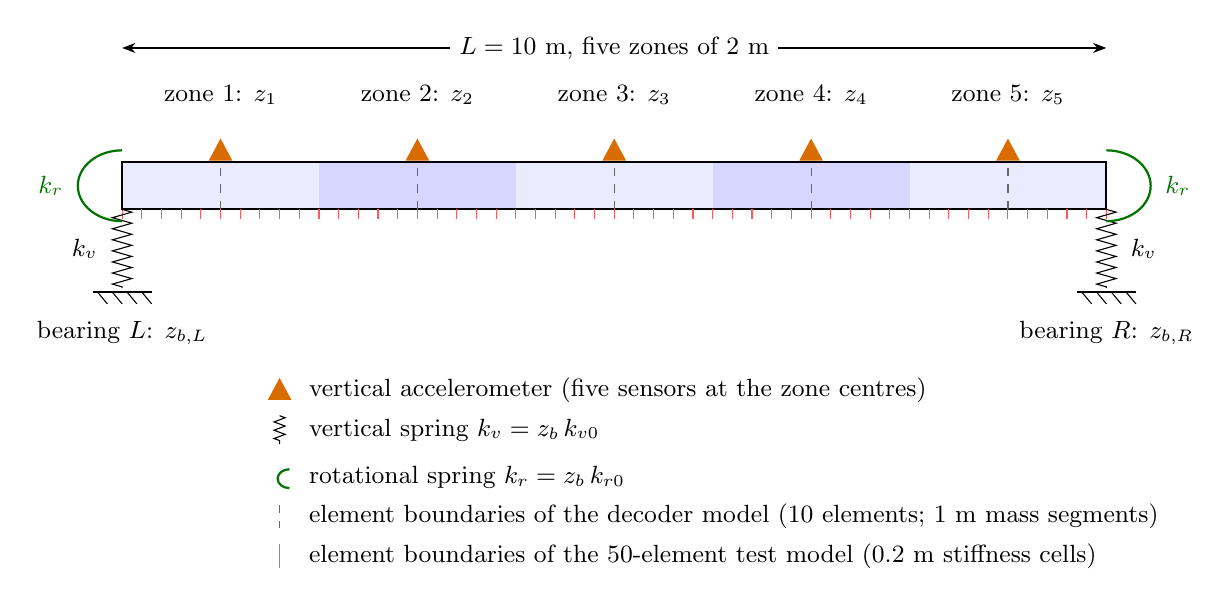
\begin{tikzpicture}[x=1.25cm,y=1cm,>=Stealth,font=\small]
  \foreach \i/\c in {0/blue!8,1/blue!16,2/blue!8,3/blue!16,4/blue!8}{
    \fill[\c] (2*\i,0) rectangle (2*\i+2,0.6);
    \node at (2*\i+1,1.45) {zone $\the\numexpr\i+1\relax$: $z_{\the\numexpr\i+1\relax}$};
  }
  \draw[thick] (0,0) rectangle (10,0.6);
  \foreach \x in {1,3,5,7,9} \draw[dashed,gray!80!black] (\x,0) -- (\x,0.6);
  \foreach \k in {0,...,50} \draw[red!65] (\k*0.2,-0.12) -- (\k*0.2,0);
  \foreach \x in {1,3,5,7,9}
    \fill[orange!85!black] (\x-0.12,0.62) -- (\x+0.12,0.62) -- (\x,0.9) -- cycle;
  \foreach \x/\lab/\a/\b in {0/{L}/90/270,10/{R}/-90/90}{
    \draw[decorate,decoration={zigzag,segment length=4,amplitude=3.5}] (\x,0) -- (\x,-1.0);
    \draw[thick] (\x-0.3,-1.05) -- (\x+0.3,-1.05);
    \foreach \h in {-0.25,-0.1,0.05,0.2} \draw (\x+\h,-1.05) -- (\x+\h+0.1,-1.2);
    \draw[thick,green!45!black] (\x,0.3) ++(\a:0.45) arc (\a:\b:0.45);
    \node[align=center,anchor=north] at (\x,-1.3) {bearing $\lab$: $z_{b,\lab}$};
  }
  \node[anchor=east] at (-0.15,-0.5) {$k_v$};
  \node[anchor=east,green!45!black] at (-0.5,0.3) {$k_r$};
  \node[anchor=west] at (10.15,-0.5) {$k_v$};
  \node[anchor=west,green!45!black] at (10.5,0.3) {$k_r$};
  \draw[<->] (0,2.05) -- (10,2.05) node[midway,fill=white] {$L=10$ m, five zones of 2 m};
  \begin{scope}[shift={(1.6,-2.3)}]
    \fill[orange!85!black] (-0.12,-0.12) -- (0.12,-0.12) -- (0,0.16) -- cycle;
    \node[anchor=west] at (0.2,0) {vertical accelerometer (five sensors at the zone centres)};
    \draw[decorate,decoration={zigzag,segment length=3,amplitude=2}] (0,-0.32) -- (0,-0.68);
    \node[anchor=west] at (0.2,-0.5) {vertical spring $k_v=z_b\,k_{v0}$};
    \draw[thick,green!45!black] (0.1,-1.0) arc (90:270:0.12);
    \node[anchor=west] at (0.2,-1.1) {rotational spring $k_r=z_b\,k_{r0}$};
    \draw[dashed,gray!80!black] (0,-1.45) -- (0,-1.75);
    \node[anchor=west] at (0.2,-1.6) {element boundaries of the decoder model (10 elements; 1 m mass segments)};
    \draw[red!65] (0,-1.95) -- (0,-2.25);
    \node[anchor=west] at (0.2,-2.1) {element boundaries of the 50-element test model (0.2 m stiffness cells)};
  \end{scope}
\end{tikzpicture}
\caption{Revised case study: beam on elastic bearings. The seven unknowns are the stiffness reduction factors of the
five deck zones ($z_1,\dots,z_5$) and of the two bearings ($z_{b,L}$, $z_{b,R}$, which scale both springs of each
bearing). The decoder of the VAE uses the nominal 10-element model; the test structures are also computed with a
50-element model.}
\label{fig:bridge}
\end{figure}

\begin{table}[H]
\centering\small
\caption{Main specifications of the revised case study.}
\label{tab:specs}
\begin{tabular}{p{3.9cm}p{11cm}}
\toprule
Deck & $L=10$ m, $E=210$ GPa, $\rho=7850$ kg/m$^3$, $A=0.005$ m$^2$, $I=8.33\times10^{-6}$ m$^4$ \\
Bearings (each end) & laminated elastomeric pad: $k_{v0}=3.6\times10^{7}$ N/m, $k_{r0}=6.8\times10^{4}$ N\,m/rad \\
Unknowns (latent space) & $\z\in[0.45,1]^7$: five deck zones and two bearings \\
Decoder model & 10 elements (2 per zone), 22 DOFs, nominal mass \\
Data-generating models & as-built structures computed with 10 elements (training, validation and test) and with 50
elements (second test set), 102 DOFs \\
Observations & first four frequencies (3.56, 13.46, 29.81 and 52.39 Hz for the healthy bridge) and vertical mode
shapes at five sensors \\
Measurement noise & 2.5\% on the frequencies; 5\% of the peak amplitude on the mode-shape components \\
Modelling error & mass of each 1 m segment: $\mathcal{N}(0,0.05^2)$; flexibility of each 0.2 m cell:
$\mathcal{N}(0,0.025^2)$ with zero mean in each zone; FE discretization (second test set) \\
\bottomrule
\end{tabular}
\end{table}

\begin{action}
New description of the case study \lines{xx--yy}, new Fig.~\tbd{x} (Fig.~\ref{fig:bridge}) and new Table~\tbd{x}
(Table~\ref{tab:specs}); all results recomputed with the new datasets \lines{xx--yy}.
\end{action}

% =============================================================================
\section{Reviewer \#1}
% =============================================================================

\begin{rcomment}{}
This paper presents a physics-informed Gaussian copula variational autoencoder for uncertainty-aware damage
identification using noisy natural frequencies and mode shapes. Replacing the learned decoder with a differentiable
eigensolver appears to be an interesting approach for end-to-end training, and the manuscript is clearly written. The work
builds on the authors' earlier Gaussian copula VAE (Reference 41) and extends it by embedding the eigensolver and
increasing the latent dimensionality from 2 to 5. The current validation is based on a single five-element synthetic
beam with measurement noise, and I believe that some additional evidence would further strengthen the conclusions
regarding uncertainty quantification, reliability, and scalability. Some clarifications are needed to better understand
the method and its applications.
\end{rcomment}

\begin{response}
We thank the reviewer for the positive assessment and for the constructive comments. Following them, the revised
study is no longer based on a single five-element beam with measurement noise: the structure rests on elastic bearings,
the latent space has seven variables, the data include modelling errors, and the trained model is tested on data from
two FE models. The responses below describe these changes.
\end{response}

% -----------------------------------------------------------------------------
\begin{rcomment}{1}
The training and test data are generated using the same five-element model. Could the authors consider testing the
trained model on observations generated from a finer mesh while retaining the same five damage zones and sensor
locations as in the current paper? This would help assess robustness to model-form uncertainty, since field observations
may not necessarily be well represented by such a coarse discretization.
\end{rcomment}

\begin{response}
We agree that generating training and test data with the model embedded in the decoder is a favourable setting, and
we have followed the reviewer's suggestion.

\textit{Decoder model.} Before testing on finer-mesh data, we checked whether the model embedded in the decoder is
accurate enough. With one element per zone (the discretization of the submitted version), the error of the fourth
frequency is 2.3\% and that of the fifth is 10.2\% with respect to a converged model (Table~\ref{tab:mesh}). Such errors are comparable to or
larger than the identification noise, so a finer-mesh test would mainly measure the discretization error of the
decoder. We therefore embed a 10-element model (two elements per zone) in the decoder; its error is below 0.17\% for the
four modes used. The latent variables are still one stiffness factor per damage zone (plus one per bearing, see R2.2),
whatever the number of elements:
\begin{equation}
\hat{\mathbf{K}}_{\mathrm{G}}(\z)=\sum_{k=1}^{5} z_k\sum_{e\in\mathcal{Z}_k}\mathbf{K}_{e}
+z_{b,L}\,\mathbf{K}_{b,L}+z_{b,R}\,\mathbf{K}_{b,R},
\label{eq:Kz}
\end{equation}
where $\mathcal{Z}_k$ is the set of elements of zone $k$ and $\mathbf{K}_{b,L}$, $\mathbf{K}_{b,R}$ contain the nominal
bearing springs.

\textit{Two test sets with the same structures.} The test set contains 1\,200 as-built structures (damage condition and
as-built deviations, see R1.2). Each of them is observed twice: the set ``test'' is computed with the 10-element model
(the discretization of the decoder), and the set ``test-fine'' with a 50-element model (ten elements per zone), with the
same five damage zones and the same five sensors. Both sets use the same measurement-noise realizations. Hence, the FE
discretization is the only difference between them, and any change in the results is due to model-form error. The
sensors are now placed at the zone centres instead of the zone boundaries (see R3.4).

\textit{Results so far.}
\begin{itemize}[leftmargin=*]
\item On average over the test structures, the frequencies of the 50-element model differ from those of the decoder
by $-0.001\%$ (mode 1) to $-0.17\%$ (mode 4), i.e., less than 7\% of the identification noise, and the mode shapes at the
sensors are indistinguishable ($1-\mathrm{MAC}<10^{-6}$; Table~\ref{tab:budget}).
\item The likelihood calibrated on 10-element data remains calibrated on 50-element data: at the true damage condition,
the frequency term of the likelihood equals 1.009 (test) and 0.986 (test-fine) times its theoretical value
(Fig.~\ref{fig:calib}).
\item The exact posteriors (computed with sequential Monte Carlo, see R1.3) obtained from both test sets are almost
identical. For the benchmark scenarios P3, P6, P7 and P9, their means differ by at most 0.006, their standard deviations
by at most 3\%, and the mean Wasserstein distance between marginals is below 0.004 (Fig.~\ref{fig:testfine}).
\item VAE metrics on both test sets: \tbd{Table with MSE, MAE, ALL, MACE and coverage on test and test-fine}.
\end{itemize}
\end{response}

\begin{table}[H]
\centering\small
\caption{Relative error (\%) of the natural frequencies of the healthy bridge with respect to a 200-element model.}
\label{tab:mesh}
\begin{tabular}{lccccc}
\toprule
Model & $f_1$ & $f_2$ & $f_3$ & $f_4$ & $f_5$ \\
\midrule
5 elements (discretization of the submitted version) & 0.012 & 0.171 & 0.798 & 2.318 & 10.247 \\
10 elements (decoder) & 0.001 & 0.011 & 0.053 & 0.163 & 0.382 \\
50 elements (test-fine) & 0.000 & 0.000 & 0.000 & 0.000 & 0.001 \\
\midrule
Frequencies of the 200-element model [Hz] & 3.555 & 13.457 & 29.807 & 52.389 & 80.868 \\
\bottomrule
\end{tabular}
\end{table}

\begin{figure}[H]
\centering
\begin{subfigure}{0.49\textwidth}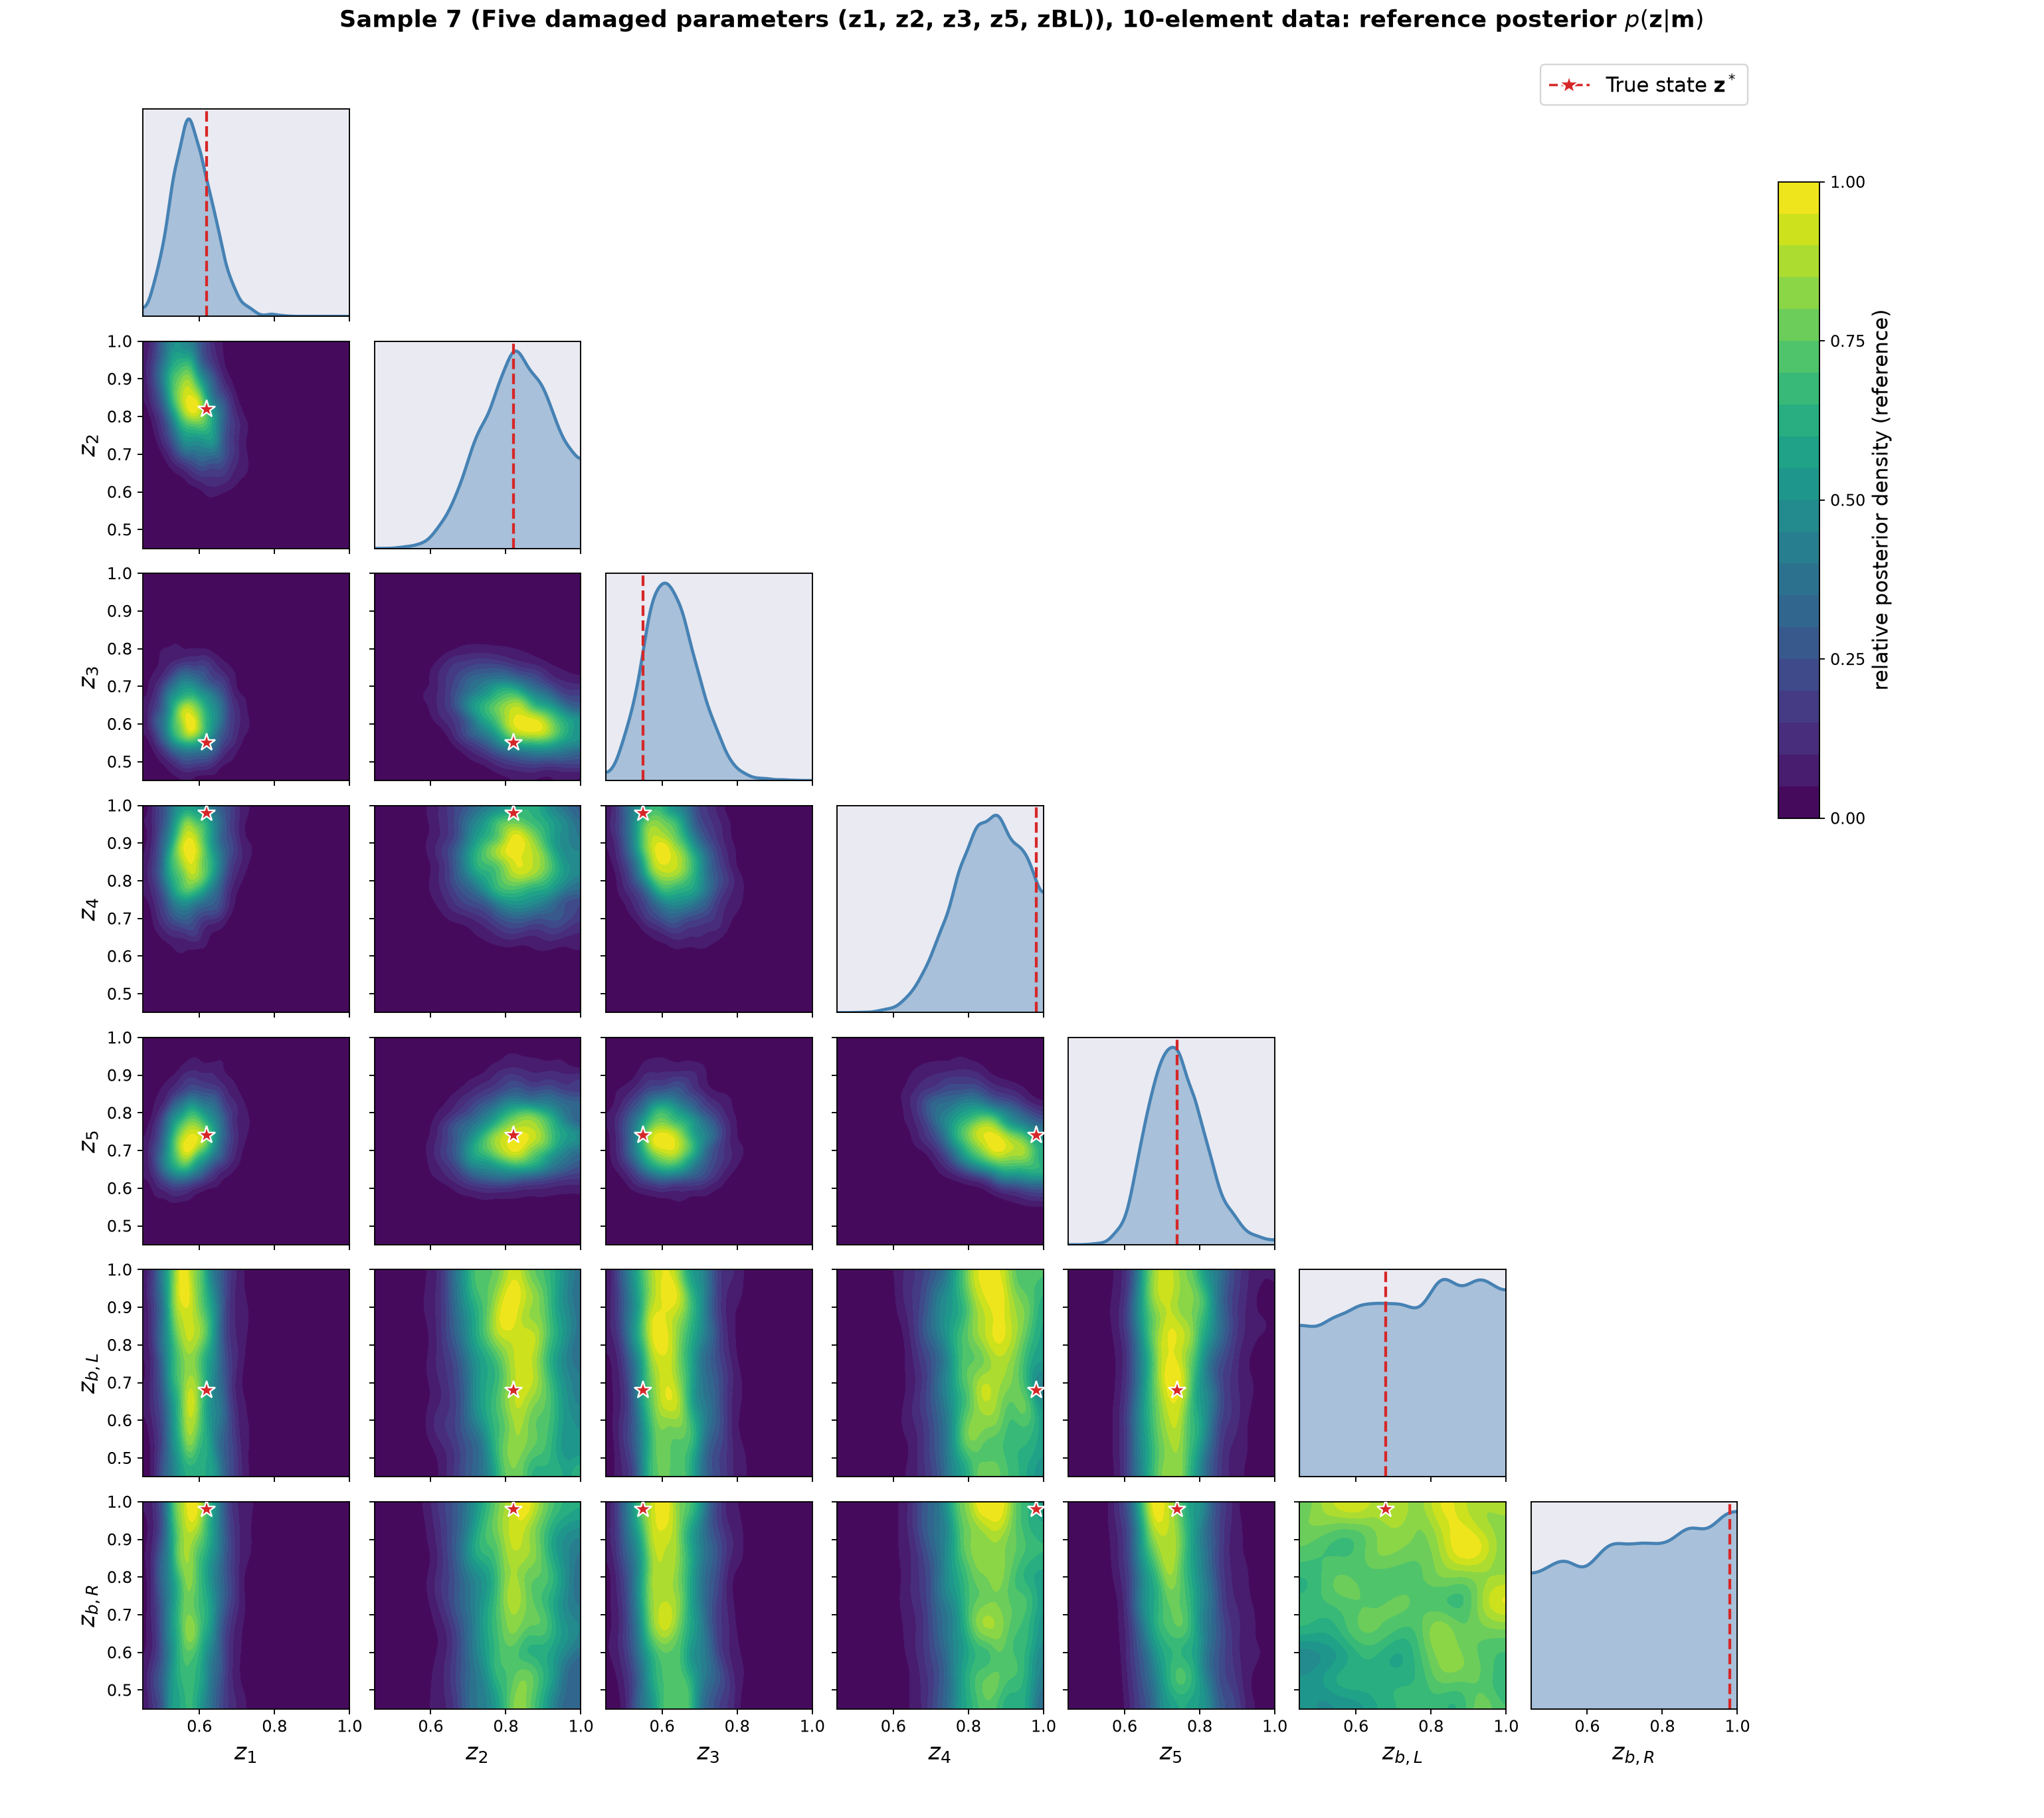
\includegraphics[width=\textwidth]{figures_v6/Fig_reference_posterior_P7_test.png}
\caption{Data from the 10-element model (test)}\end{subfigure}
\begin{subfigure}{0.49\textwidth}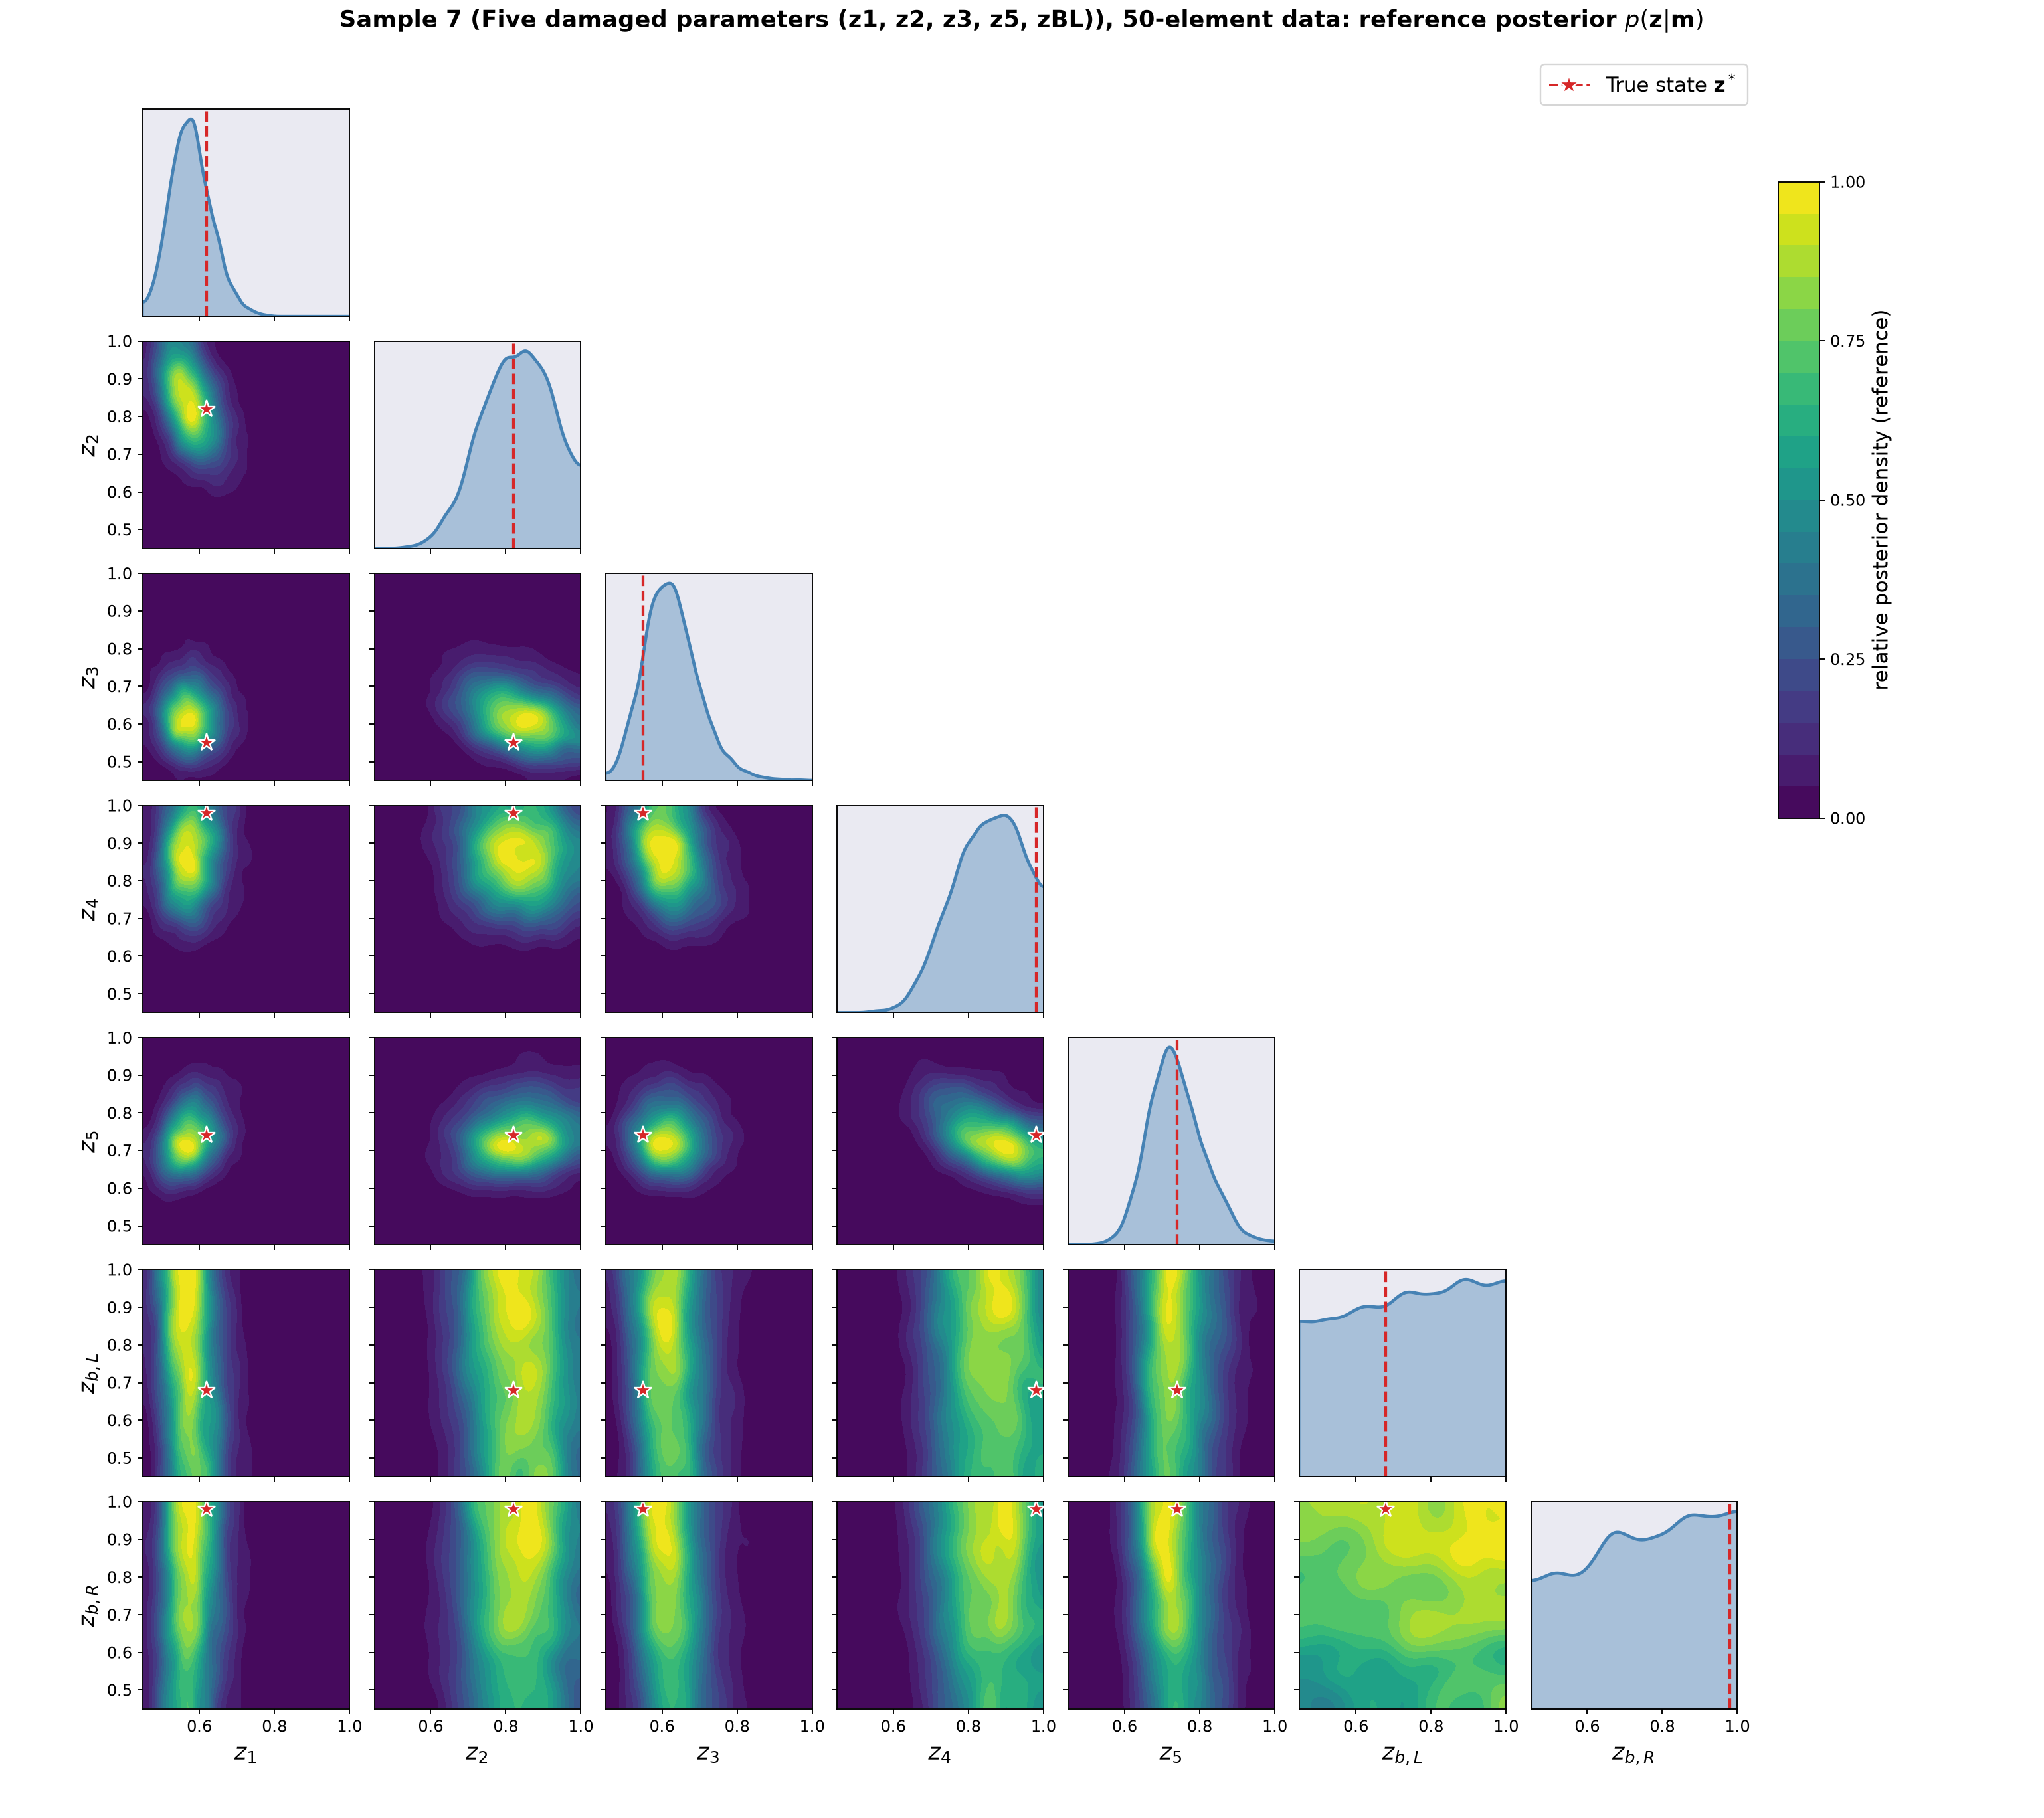
\includegraphics[width=\textwidth]{figures_v6/Fig_reference_posterior_P7_test_fine.png}
\caption{Data from the 50-element model (test-fine)}\end{subfigure}
\caption{Exact posterior of benchmark P7 (five damaged parameters) computed from the two observations of the same
as-built structure. The red star marks the true damage condition.}
\label{fig:testfine}
\end{figure}

\begin{action}
The decoder now embeds a 10-element model \lines{xx--yy}; a second test set generated with a 50-element model is
described in \lines{xx--yy}, and Table~\tbd{x} reports the metrics on both test sets.
\end{action}

% -----------------------------------------------------------------------------
\begin{rcomment}{2}
The introduction identifies model uncertainty, measurement error, and environmental variability as sources of
ill-posedness, whereas the numerical study focuses primarily on measurement noise. It would be useful to investigate how
the proposed framework handles the other sources of uncertainty or, alternatively, to discuss this point more explicitly
as a limitation of the present study.
\end{rcomment}

\begin{response}
We agree. The revised study includes, in every dataset (training, validation and both test sets), the two sources of
uncertainty that can be represented realistically in a synthetic setting: measurement error and modelling error.

\textit{Measurement error.} As in the submitted version, we add 2.5\% noise to the identified frequencies and noise with
a standard deviation of 5\% of the peak amplitude to each mode-shape component.

\textit{Modelling error.} Each measurement comes from an as-built structure that differs from the nominal FE model
embedded in the decoder:
\begin{itemize}[leftmargin=*]
\item \emph{Mass}: the mass of each 1 m segment is multiplied by $1+\mu_s$, with $\mu_s\sim\mathcal{N}(0,0.05^2)$
(non-structural mass, pavement, tolerances of the cross-sections).
\item \emph{Stiffness variability within each zone}: the flexibility of each 0.2 m cell is multiplied by
$1+\varepsilon_c$, with $\varepsilon_c\sim\mathcal{N}(0,0.025^2)$ and zero mean inside each zone, so that the
equivalent stiffness of the zone remains $z_k$.
\item \emph{Discretization}: the second test set is computed with a 50-element model (R1.1).
\end{itemize}
The element matrices of an as-built structure are therefore
\begin{equation}
\mathbf{M}_e^{\mathrm{ab}}=(1+\mu_{s(e)})\,\mathbf{M}_e,\qquad
\mathbf{K}_e^{\mathrm{ab}}=\frac{z_{k(e)}}{1+\bar{\varepsilon}_e}\,\mathbf{K}_e ,
\label{eq:asbuilt}
\end{equation}
where $s(e)$ is the segment and $k(e)$ the zone of element $e$, and $\bar{\varepsilon}_e$ is the mean flexibility
deviation of the cells of the element. Since the deviations are defined on a grid that does not depend on the mesh,
both test sets describe the same physical structures. The decoder keeps the nominal model: the realizations of these
deviations are never available to the VAE.

\textit{How the inference handles them.} We write the observations as
\begin{equation}
\m=\mathbf{g}(\z)+\bm{\delta}_{\mathrm{model}}+\bm{\epsilon}_{\mathrm{meas}},
\label{eq:discrepancy}
\end{equation}
where $\mathbf{g}(\z)$ are the modal properties of the nominal model. If the likelihood ignored
$\bm{\delta}_{\mathrm{model}}$, the stiffness factors would have to absorb the modelling error, which biases the
estimates and makes the posterior overconfident. Instead, we estimate the statistics of
$\bm{\delta}_{\mathrm{model}}+\bm{\epsilon}_{\mathrm{meas}}$ by simulating 6\,000 as-built structures with new random
deviations, and include them in the likelihood: a full covariance matrix of the log-frequency errors (standard
deviations 2.66--2.68\%, of which about 0.95\% is due to the modelling error; correlation 0.09 between modes) and a
standard deviation per mode for the mode-shape errors (0.031--0.035). This is the standard treatment of model
discrepancy in Bayesian FE model updating, and it leaves the architecture unchanged. We verified the calibration on
independent data: at the true damage condition, every likelihood term equals 0.986--1.01 times its theoretical value
(Fig.~\ref{fig:calib}). Table~\ref{tab:budget} and Fig.~\ref{fig:budget} quantify each source: the mass deviations are
the dominant modelling error (about 0.95\% on the frequencies and up to $1.0\times10^{-3}$ in $1-\mathrm{MAC}$ for
mode~4), while the finer mesh only introduces a small systematic shift (at most 0.17\%).

\textit{Environmental variability.} We do not simulate environmental effects. Their influence on the modal properties
depends strongly on the structure (for instance, the stiffening of the pavement and of the bearings below freezing), and
a realistic description requires long-term monitoring data with measured temperatures. We now discuss this explicitly
as a limitation. The framework can incorporate such effects either as an additional, correlated term of
$\bm{\delta}_{\mathrm{model}}$ in Eq.~\eqref{eq:discrepancy}, or by feeding the measured temperature to the encoder; we
indicate this as future work with field data.
\end{response}

\begin{table}[H]
\centering\small
\caption{Size of each source of discrepancy between the measurements and the nominal decoder (modes 1 to 4), over the
test damage states: mean and standard deviation of $\log f_{\mathrm{data}}-\log f_{\mathrm{decoder}}$ and mean
$1-\mathrm{MAC}$ of the vertical mode shapes.}
\label{tab:budget}
\begin{tabular}{lccc}
\toprule
Source & Mean $\Delta\log f$ (\%) & Std $\Delta\log f$ (\%) & Mean $1-\mathrm{MAC}$ \\
\midrule
Finer mesh (50 elements) & $-0.001$ to $-0.165$ & $<0.005$ & $<10^{-6}$ \\
Mass (5\% per 1 m segment) & 0.010 to 0.030 & 0.91--0.98 & up to $1.0\times10^{-3}$ \\
Within-zone stiffness (2.5\%) & $<0.002$ & 0.04--0.09 & $<10^{-5}$ \\
Measurement noise & $\approx0$ & 2.45--2.50 & $3.6$--$4.0\times10^{-3}$ \\
\bottomrule
\end{tabular}
\end{table}

\begin{figure}[H]
\centering
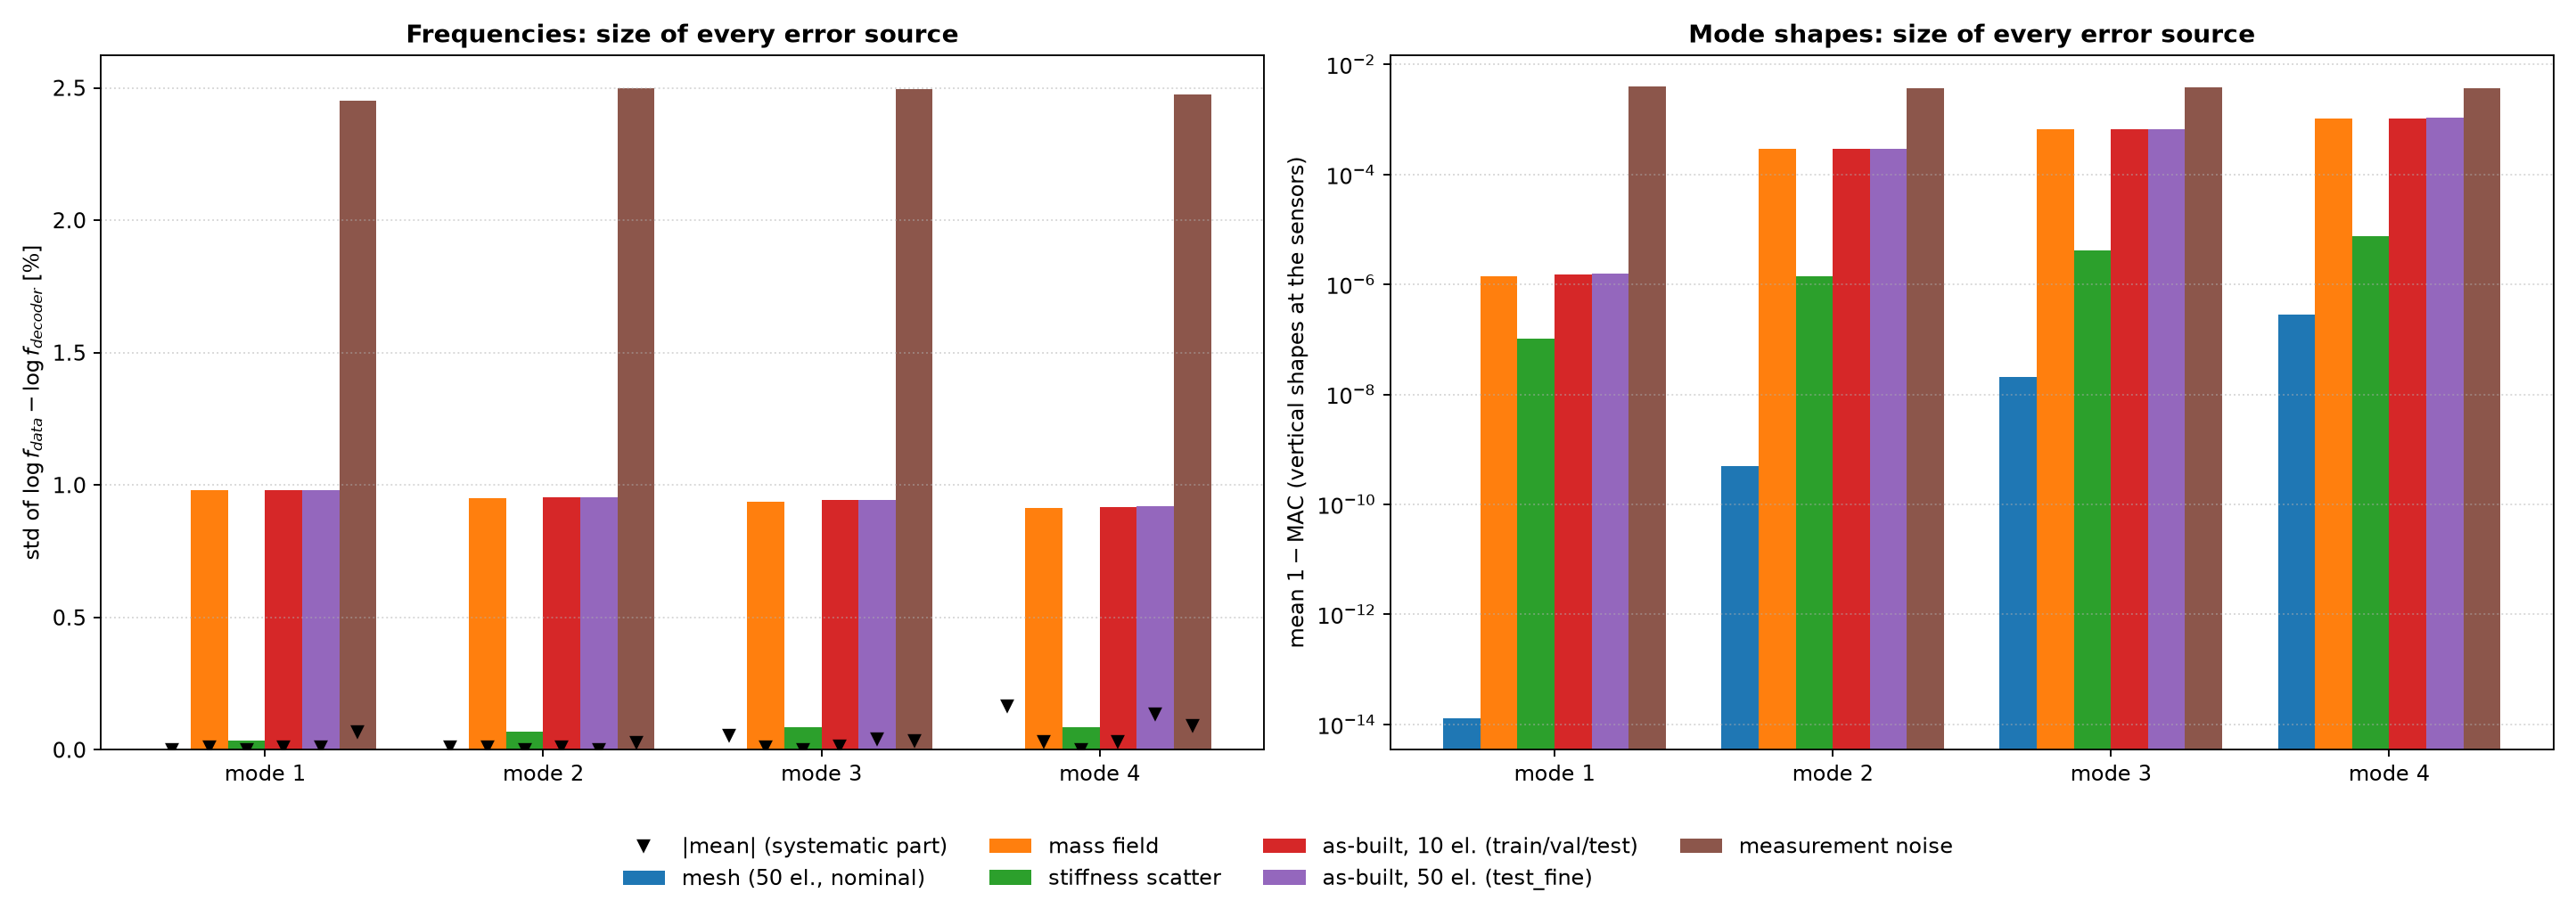
\includegraphics[width=\textwidth]{figures_v6/Fig_model_error_budget.png}
\caption{Size of each source of discrepancy between the measurements and the nominal decoder, per mode: frequencies
(left) and vertical mode shapes (right).}
\label{fig:budget}
\end{figure}

\begin{figure}[H]
\centering
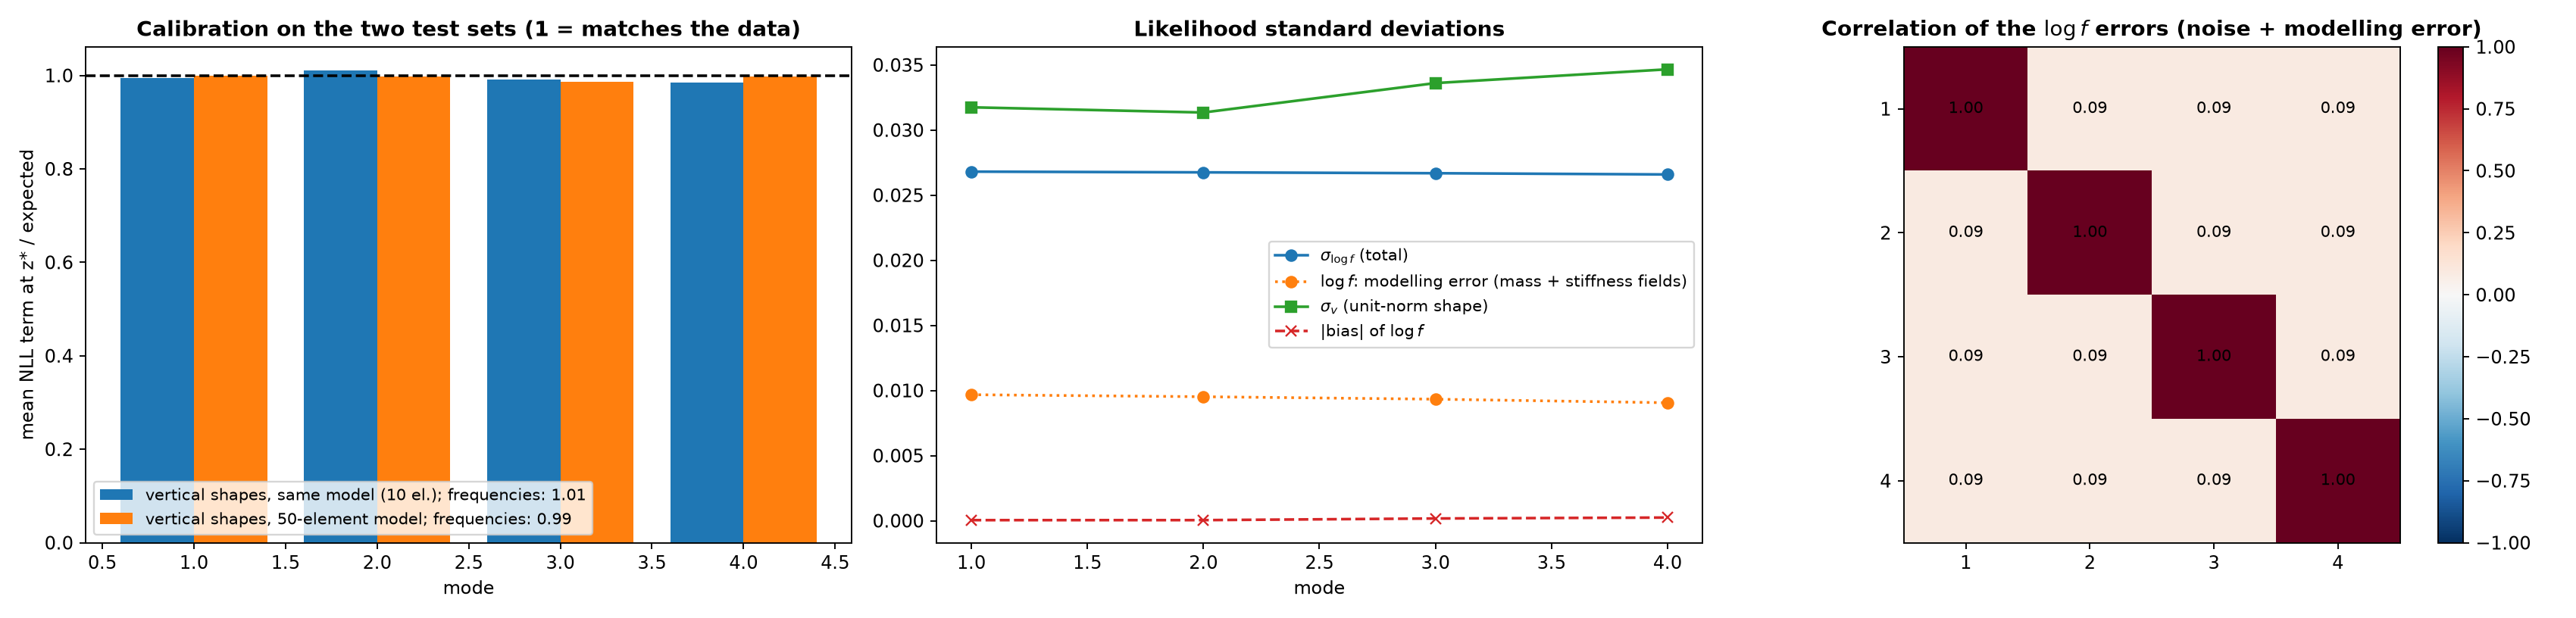
\includegraphics[width=\textwidth]{figures_v6/Fig_likelihood_calibration.png}
\caption{Calibration of the likelihood. Left: average likelihood terms at the true damage condition divided by their
theoretical value, for both test sets (1 means calibrated). Centre: standard deviations of the log-frequencies and of
the unit-norm vertical mode shapes. Right: correlation between the log-frequency errors of different modes.}
\label{fig:calib}
\end{figure}

\begin{action}
New subsection on the sources of uncertainty and their treatment in the likelihood \lines{xx--yy}, with
Eqs.~\eqref{eq:asbuilt}--\eqref{eq:discrepancy}, Table~\ref{tab:budget} and Figs.~\ref{fig:budget}--\ref{fig:calib};
environmental variability discussed as a limitation in the conclusions \lines{xx--yy}.
\end{action}

% -----------------------------------------------------------------------------
\begin{rcomment}{3}
The abstract reports 77.2\% coverage (line 32), whereas line 352 reports a value of 0.789 for nominal 95\% intervals.
Could the authors clarify how these two values are related? A value below 80\% for nominal 95\% intervals may indicate
some undercoverage. A brief discussion of how the uncertainty intervals are calibrated would therefore be helpful.
\end{rcomment}

\begin{response}
We thank the reviewer for pointing out this inconsistency. The two values were obtained in two different evaluation
runs of the submitted version, and the abstract was not updated after the final run.
\authornote{please confirm the origin of 77.2\% and 0.789.} In the revised manuscript, a single coverage value is
reported, the abstract and the text use the same value, and the definition of the intervals is stated explicitly.

The reviewer is right that these values indicate undercoverage. We identified two causes:
\begin{enumerate}[leftmargin=*]
\item \emph{The width of the approximate posterior was not calibrated.} In the submitted loss, the frequency and MAC
terms had fixed weights ($\lambda=10$) that were not derived from the noise statistics, and the entropy term was
scaled by $\gamma^2$, with $\gamma=0.30$ selected to balance point accuracy and distributional quality. The minimizer of such a loss is a tempered posterior
whose width depends on these weights, so its credible intervals cannot be expected to reach their nominal coverage.
\item \emph{Equal-tailed intervals and the upper bound $z=1$.} An undamaged parameter lies close to the upper bound of
the support, where its posterior accumulates. An equal-tailed (central) 95\% interval excludes the upper 2.5\% of the
probability, and therefore often excludes a true value close to 1, even when the posterior is correct. In the revised
test set, 67\% of the parameters are undamaged ($z^*\ge0.95$) and 18\% lie above the 97.5\% quantile of the prior. As a
result, even the prior, which ignores the data, reaches only 81\% coverage with central 95\% intervals on this test set.
A coverage of central intervals below 80\% is therefore not necessarily a sign of a poorly calibrated posterior.
\end{enumerate}

We made the following changes:
\begin{itemize}[leftmargin=*]
\item \emph{Calibrated likelihood.} The data terms of the loss are the negative log-likelihood of the frequency and
mode-shape errors, with the variances calibrated by simulation and verified on independent data (R1.2):
\begin{equation}
\mathrm{NLL}(\z;\m)=\tfrac12\,\mathbf{d}^{\top}\bm{\Sigma}_f^{-1}\mathbf{d}
+\sum_{j=1}^{n_m}\frac{1-\mathrm{MAC}_j(\bm{\Phi},\hat{\bm{\Phi}}(\z))}{2\,s_{v,j}^2},\qquad
\mathbf{d}=\log\f-\mathbf{b}-\log\hat{\f}(\z).
\label{eq:nll}
\end{equation}
For unit-norm mode shapes perturbed by Gaussian noise, $1-\mathrm{MAC}_j$ equals the squared noise component
perpendicular to the shape, so the second term is the Gaussian log-likelihood of that component.
\item \emph{No tempering ($\gamma=1$).} With a uniform prior on $\mathcal{S}=[0.45,1]^7$, the loss
\begin{equation}
\mathcal{L}(\bm\theta)=\frac1N\sum_{i=1}^N\Big(\mathbb{E}_{q}\big[\mathrm{NLL}(\z;\m_i)\big]
-\gamma^2\,\mathcal{H}\big[q_{\bm\zeta_{\bm\theta}}(\z|\m_i)\big]\Big)
\label{eq:loss}
\end{equation}
is the negative ELBO for $\gamma=1$ (up to a constant), and its minimizer is the Bayesian posterior within the
variational family. $\mathcal{H}$ is the entropy of the copula model: the copula part, $\frac12\log\det\mathbf{R}$, is
computed exactly, and only the entropies of the marginals are estimated with the samples.
\item \emph{Exact credible intervals.} The marginals of the approximate posterior are Kumaraswamy mixtures with a
closed-form CDF $F_{q,e}$, so we compute the probability integral transform $u_{t,e}=F_{q,e}(z^*_{t,e})$ of every true
value exactly. The true value lies inside the equal-tailed interval of level $p$ if $|2u_{t,e}-1|\le p$, and inside the
highest-density region of level $p$ if the posterior probability of $\{z: q_e(z)>q_e(z^*_{t,e})\}$ does not exceed $p$.
\item \emph{Reliability diagrams.} We compute the empirical coverage at 19 nominal levels, from $p=0.05$ to $p=0.95$ in
steps of 0.05, and the MACE, with both types of intervals, for all parameters and separately for deck zones and bearings, for damaged and
undamaged parameters, and for the test scenarios drawn from the prior, where a Bayesian posterior must be calibrated by
construction.
\item \emph{Reference posterior.} We compare the VAE with the exact posterior obtained by sequential Monte Carlo with
the same likelihood and prior. It starts from samples of the prior, introduces the likelihood gradually through an
exponent that grows from 0 to 1, and never uses the true damage condition. This separates the approximation error of
the VAE from the effect of the bounds described above.
\end{itemize}

\tbd{Results of the final training: coverage and MACE with both types of intervals (all, deck zones, bearings,
damaged, undamaged, scenarios drawn from the prior), reliability diagram, and comparison with the exact posteriors of
the benchmark scenarios.}
\end{response}

\begin{action}
Abstract and Section~\tbd{x} corrected so that they report the same value \lines{xx--yy}; new paragraph on the
calibration of the likelihood and the definition of the intervals \lines{xx--yy}; new reliability diagram (Fig.~\tbd{x})
and coverage table (Table~\tbd{x}).
\end{action}

% -----------------------------------------------------------------------------
\begin{rcomment}{4}
References 39 (Gaussian mixture autoencoder) and 41 (Gaussian copula VAE) introduce closely related methods that could
potentially serve as useful baselines. A comparison with these approaches would help assess the benefits of the proposed
strategy more effectively.
\end{rcomment}
\pending

% -----------------------------------------------------------------------------
\begin{rcomment}{5}
All test cases appear to be sampled from the same distribution as the training data. It would be helpful to include
several additional cases where the test data fall outside the training distribution to illustrate how the proposed
method behaves under distribution shift.
\end{rcomment}
\pending
\authornote{the test-fine set (R1.1) is a shift of the data-generating model; shifts of the damage distribution (e.g.,
$z$ below 0.45, damage outside the zones) are still to be added.}

% -----------------------------------------------------------------------------
\begin{rcomment}{6}
The paper introduces damage by sampling from a uniform distribution (line 323), which appears to result in substantial
stiffness reduction in most or all five elements simultaneously. Since structural damage is often localized, it would be
valuable to also evaluate healthy cases and cases with mild damage affecting only one or two elements. Reporting the
corresponding false-positive behavior would further support the manuscript's emphasis on early damage identification.
\end{rcomment}

\begin{response}
We agree with the reviewer. The revised design of experiments (DoE) is a stratified mixture of scenario categories
(Table~\ref{tab:doe}, Fig.~\ref{fig:doe}): healthy structures, one, two, three, or four to five damaged parameters, and a
category drawn uniformly over the support of the prior. Within each category, every damage location (five zones and two
bearings) and every combination of locations appears the same number of times. The severities of the damaged
parameters are stratified (Latin hypercube) over $[0.45,0.95)$, which covers mild to severe damage without gaps, and
the undamaged parameters lie in $[0.95,1]$. Every parameter is damaged in 33.2\% of the training samples. The validation
(2\,400 samples) and test (1\,200 samples) sets follow the same proportions.

The first eleven test samples are benchmark scenarios (Fig.~\ref{fig:doe}, bottom right): a healthy bridge (P0),
damage in a single zone with severe, moderate, mild and very mild severity (P1, P2, P3 and P10, the latter with
$z_4=0.90$), degradation of one bearing (P4), and combined scenarios (P5 to P9).

To quantify false positives, a parameter is declared damaged when the upper limit of its 95\% credible interval falls
below the damage threshold 0.95. We report the false-alarm rate (fraction of undamaged parameters declared damaged)
and the detection rate (fraction of parameters with $z^*<0.90$ declared damaged), for the whole test set and per
category, together with the posteriors of the healthy and mildly damaged benchmarks.
\tbd{False-alarm and detection rates of the final model; posteriors of P0, P3 and P10.}
\end{response}

\begin{table}[H]
\centering\small
\caption{Scenario categories of the design of experiments (14\,000 training samples).}
\label{tab:doe}
\begin{tabular}{lccl}
\toprule
Category & Share & Training samples & Damaged parameters \\
\midrule
Healthy & 10\% & 1\,400 & none \\
Single damage & 30\% & 4\,200 & one (each of the seven locations equally often) \\
Double damage & 25\% & 3\,500 & two (all 21 pairs) \\
Triple damage & 15\% & 2\,100 & three (all 35 triples) \\
Multiple damage & 10\% & 1\,400 & four or five (all 56 combinations) \\
Uniform & 10\% & 1\,400 & $\z\sim\mathcal{U}[0.45,1]^7$ (whole support of the prior) \\
\bottomrule
\end{tabular}
\end{table}

\begin{figure}[H]
\centering
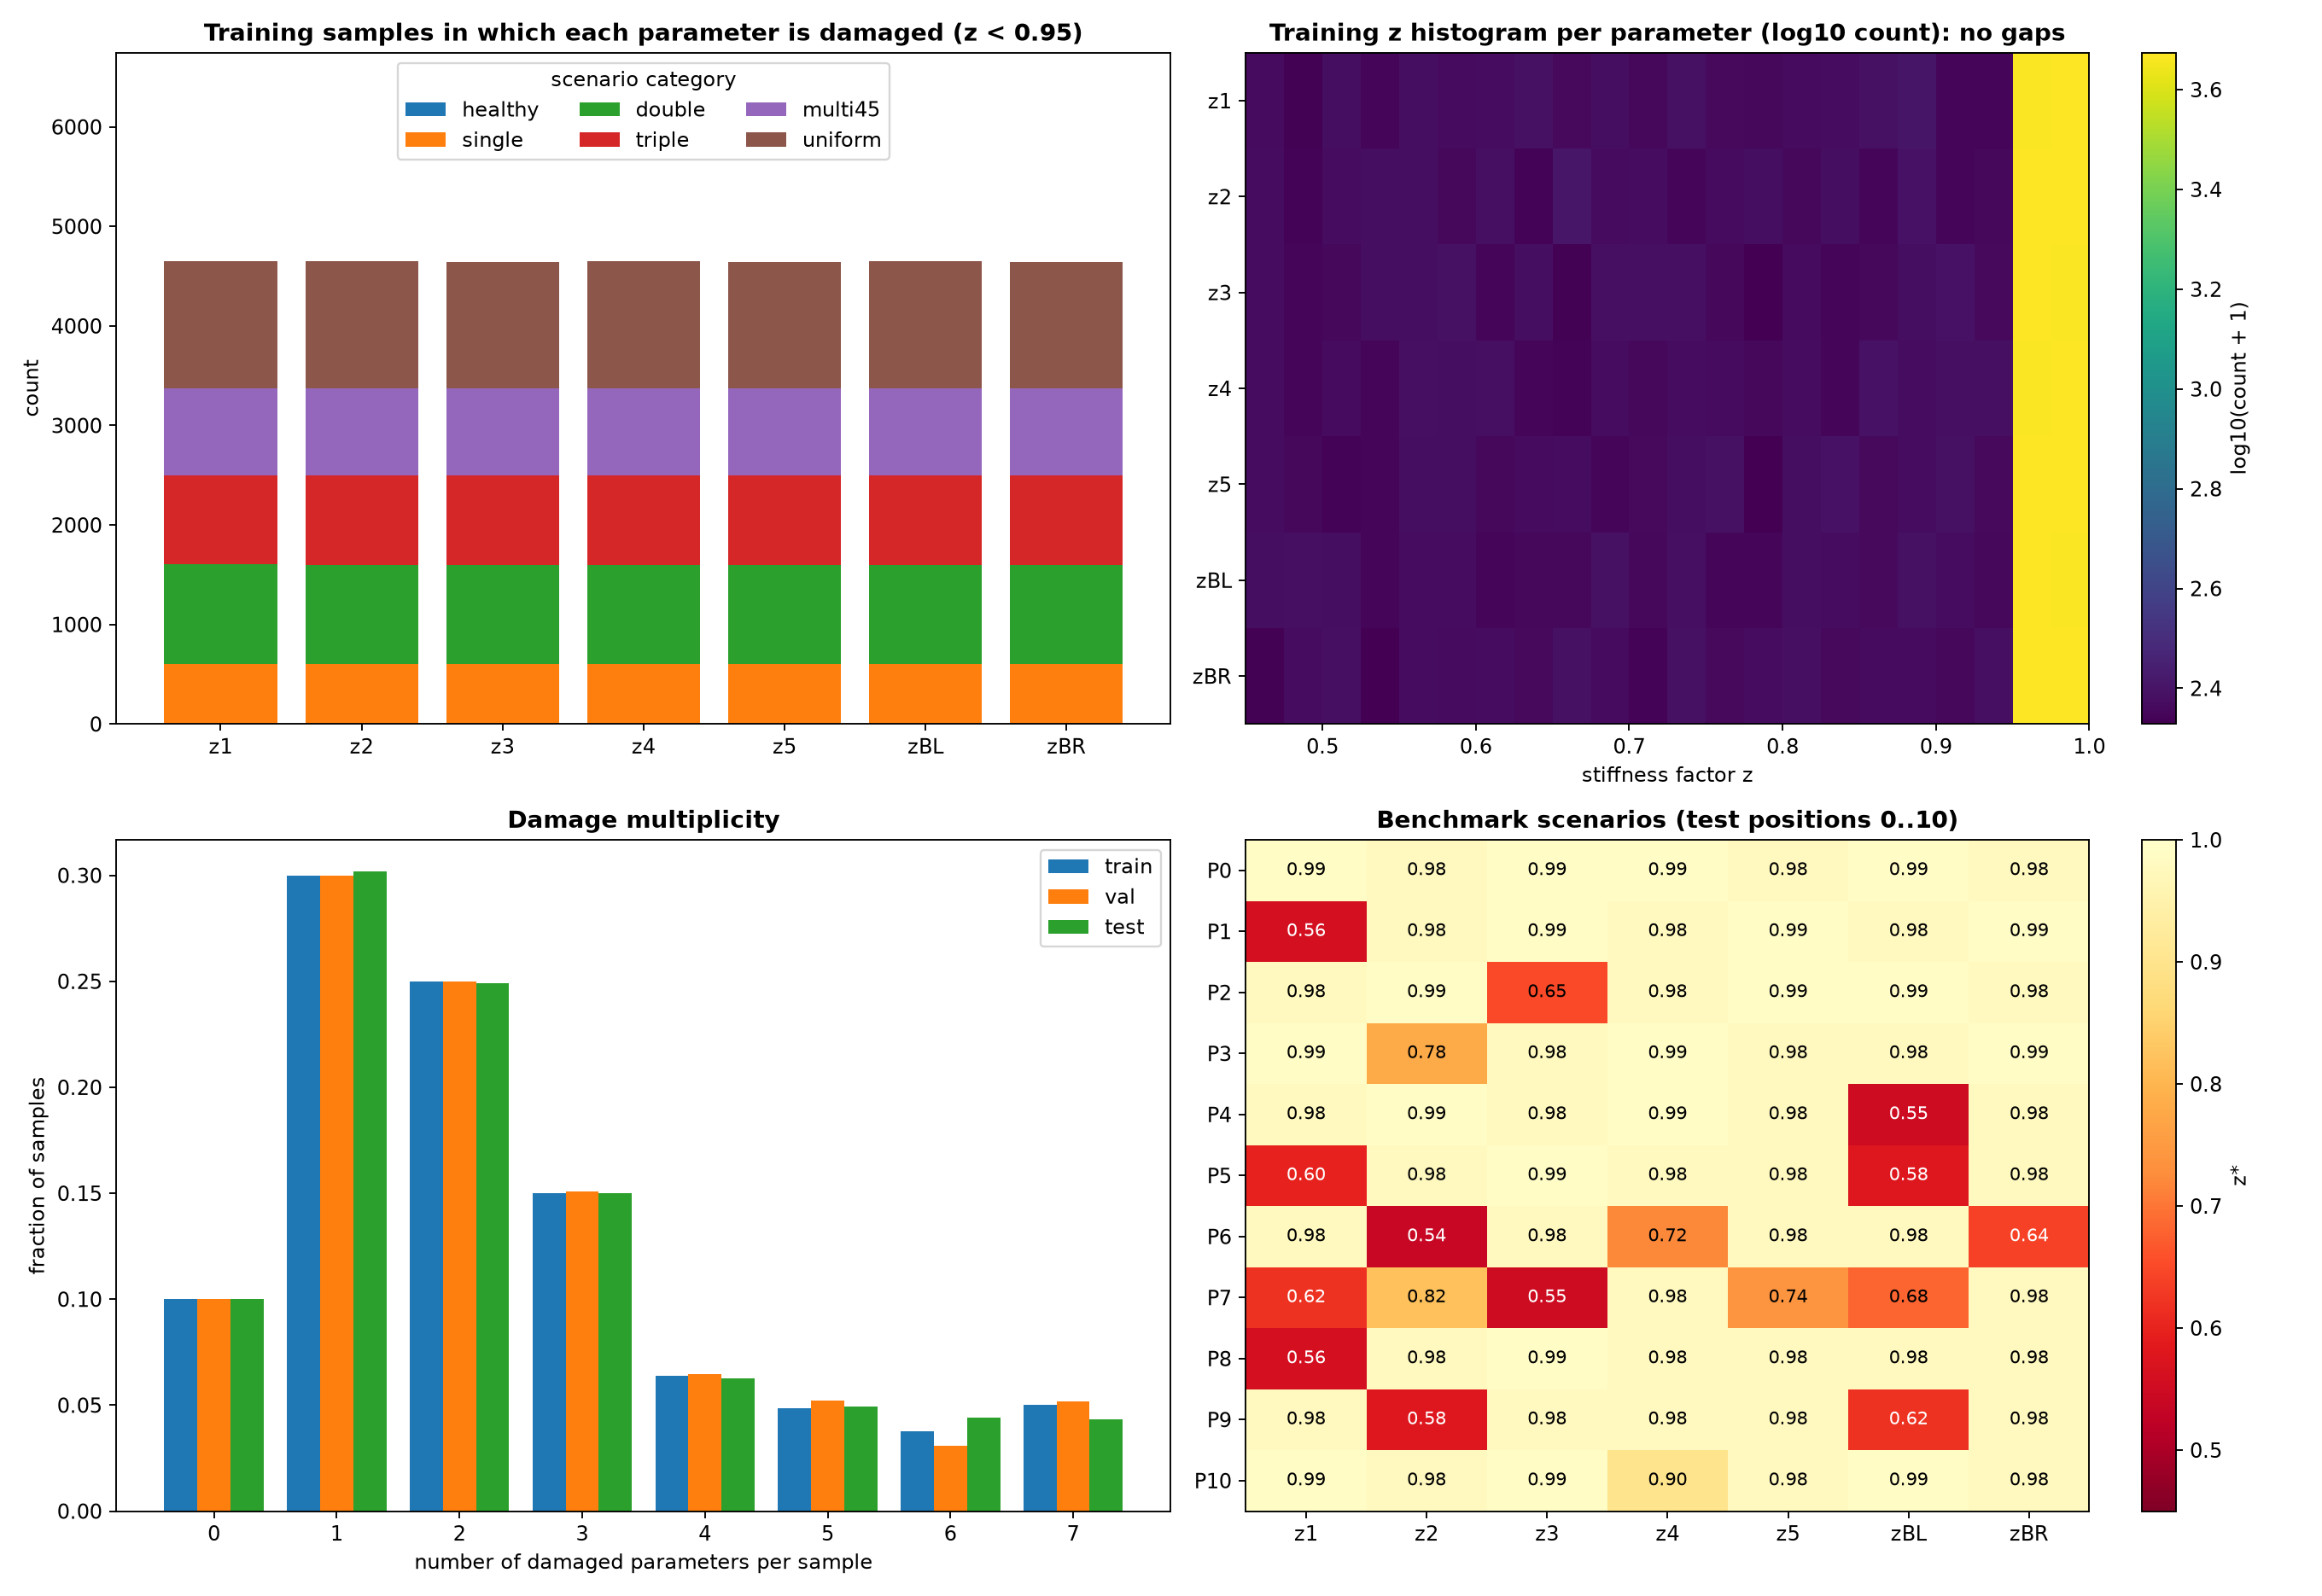
\includegraphics[width=0.95\textwidth]{figures_v6/Fig_DoE_balance.png}
\caption{Design of experiments: number of training samples in which each parameter is damaged, per category;
histogram of the stiffness reduction factors; number of damaged parameters per sample in the training, validation and
test sets; and the eleven benchmark scenarios.}
\label{fig:doe}
\end{figure}

\begin{action}
New description of the DoE \lines{xx--yy} with Table~\tbd{x} and Fig.~\tbd{x}; false-alarm and detection rates reported
in \lines{xx--yy}.
\end{action}

% -----------------------------------------------------------------------------
\begin{rcomment}{7}
How does the proposed approach perform when the system is discretized more finely? The conclusion (lines 399-403)
refers to scalability to large-scale infrastructure. Could the authors comment on the expected computational and
statistical scaling of the method for systems with hundreds of elements, particularly given that the number of copula
correlation parameters and the computational cost of the eigensolver may both increase with problem size?
\end{rcomment}

\begin{response}
In the revised formulation, the FE discretization is decoupled from the damage parametrization. The latent variables
are the stiffness factors of the damage zones and bearings, and each zone may contain any number of elements
(Eq.~\eqref{eq:Kz}). The copula has $d(d-1)/2$ correlation parameters for $d$ latent variables (21 for $d=7$), a number
that depends on the number of damage zones and not on the number of elements. In the revised study, the decoder uses 10
elements (22 DOFs) instead of 5 without changing the latent dimension, and the trained model is tested on data from a
50-element model (102 DOFs), see R1.1.

\tbd{Results of the VAE on the test-fine set.}
\end{response}
\authornote{discussion of the computational and statistical scaling still to be written: (i) structured correlation
matrices (banded, low-rank plus diagonal) keep the number of copula parameters linear in $d$; (ii) the decoder solves
one symmetric eigenproblem of size $n_{\mathrm{dof}}$ per sample, $O(n_{\mathrm{dof}}^3)$, batched; reduced-order
models or iterative solvers for the first $n_m$ modes would reduce this cost for hundreds of elements; (iii) report the
measured time per epoch for different meshes.}

\begin{action}
New paragraph on the decoupling of the mesh and the latent space \lines{xx--yy}. \tbd{scaling discussion.}
\end{action}

% -----------------------------------------------------------------------------
\begin{rcomment}{8}
A few references may benefit from a final consistency check. In particular, Reference 77 appears to contain placeholder
fields, and some references seem to be duplicated.
\end{rcomment}
\pending

% =============================================================================
\section{Reviewer \#2}
% =============================================================================

\begin{rcomment}{}
The paper presents a method based on physics-informed Gaussian copula variational autoencoder (PI-GCVAE) for
structural health monitoring (SHM) of simply supported bridges. The novelty lies in embedding a differentiable numerical
eigenvalue solver directly into the VAE architecture. The method is then demonstrated on a numerical study. The current
study is on a topic of relevance and general interest to the readers of the journal. However, I think the paper needs to
address several significant concerns and in my opinion has not yet reached the maturity to be published in CPENG
journal.
\end{rcomment}

\begin{response}
We thank the reviewer for the assessment. The concerns about the structural model motivated the main changes of the
revised case study: elastic bearings, a damage parametrization that includes the supports, two FE models, and modelling
errors in all the data. We describe them below.
\end{response}

% -----------------------------------------------------------------------------
\begin{rcomment}{1}
Introduction. The introduction is written well, but too much effort has been put on proving the methodological
novelty. I recommend focusing also on the utility to justify the value of the method for real bridges, as it seems that
the generalization of the approach is very difficult to other types of bridges considering the limitations of simply
supported bridge formulation and damage parametrization approach.
\end{rcomment}
\pending

% -----------------------------------------------------------------------------
\begin{rcomment}{2}
Methodology. The assumption of simply-supported beam for single span bridges is not realistic. The majority of them
sits on elastic bearings whose effects are demonstrated in the literature. The formulation should at least include the
vertical springs at the ends.
\end{rcomment}

\begin{response}
We agree. The revised model replaces the simple supports by elastic bearings at both ends, each represented by a
vertical spring $k_v$ and a rotational spring $k_r$ (Fig.~\ref{fig:bridge}). Since no degree of freedom is removed, the
model has $2(n_{\mathrm{el}}+1)$ DOFs. The bearings are small laminated elastomeric pads, consistent with the size of
the beam: $150\times100$ mm in plan, two 10 mm rubber layers, shear modulus $G=0.9$ MPa and shape factor $S=3$. With the
compression modulus $E_c=6GS^2=48.6$ MPa, this gives $k_{v0}=E_cA/t_r=3.6\times10^{7}$ N/m and
$k_{r0}=E_cI_p/t_r=6.8\times10^{4}$ N\,m/rad, where $A$ and $I_p$ are the area and second moment of area of the pad
and $t_r$ the total rubber thickness. \authornote{add references for the design of elastomeric bearings (e.g., AASHTO
LRFD Section 14, EN~1337-3) and for the effect of bearings on bridge dynamics.}

Each bearing has its own stiffness reduction factor, which scales both of its springs, so that damage can occur in the
deck and in the supports (Eq.~\eqref{eq:Kz}); the latent space has seven variables. The rotational springs raise the
first frequency from 3.32 Hz (simply supported) to 3.56 Hz. The vertical springs are about 400 times stiffer than the
flexural stiffness of the beam at mid-span ($48EI/L^3$): alone, they lower the first frequency by only 0.1\% with
respect to rigid supports. Consequently, a degradation of the bearings changes the four measured modes little compared
with the identification noise: even a 55\% loss of bearing stiffness shifts the frequencies by only 0.7--1.9\% (below
the 2.5\% noise) and the mode shapes by $1-\mathrm{MAC}\le1.4\times10^{-3}$ (below the noise level of about
$4\times10^{-3}$), and its effect resembles a slight softening of the adjacent end zone. Therefore, the exact posteriors of the bearing factors remain close to the prior (standard
deviation 0.15--0.16, versus 0.16 for the prior), whereas the deck zones are identified with standard deviations of
0.04--0.09. The framework reports this lack of information as a wide posterior instead of a spurious point estimate.

\textit{Physical explanation.} The sensitivity of the squared frequency of a mode to the stiffness of a spring equals
the fraction of the modal strain energy stored in that spring. Table~\ref{tab:bearing_energy} shows these fractions for
the bearings of our bridge. The laminated pads are very stiff in compression compared with the span
($k_{v0}L^3/EI\approx2\times10^4$), so the supports barely move vertically and the vertical springs store less than
4\% of the energy of any mode. The pads are designed to allow rotation ($k_{r0}L/EI=0.39$), so the rotational springs
provide only a partial fixity, which matters for the first mode (13\% of its energy) and much less for the higher ones.
In addition, the mode shapes are measured on the deck, where the bearings have little effect, and a softer bearing
produces changes similar to those of a slightly softer end zone. This insensitivity is a property of the vertical
bending modes of a bridge on elastomeric bearings, not of the identification method; we did not modify the model to
increase it artificially.
\end{response}

\begin{table}[H]
\centering\small
\caption{Share of the modal strain energy stored in the bearings, and change of the frequencies when one bearing loses
55\% of its stiffness ($z_{b,L}=0.45$).}
\label{tab:bearing_energy}
\begin{tabular}{lcccc}
\toprule
 & Mode 1 & Mode 2 & Mode 3 & Mode 4 \\
\midrule
Energy in the vertical springs (\%) & 0.2 & 0.8 & 1.8 & 3.3 \\
Energy in the rotational springs (\%) & 12.7 & 3.6 & 1.6 & 0.9 \\
Frequency change, $z_{b,L}=0.45$ (\%) & $-1.9$ & $-0.7$ & $-0.8$ & $-1.2$ \\
\midrule
Identification noise of the frequencies (\%) & 2.5 & 2.5 & 2.5 & 2.5 \\
\bottomrule
\end{tabular}
\end{table}

\begin{action}
New FE model with elastic bearings and seven unknowns \lines{xx--yy}, Fig.~\tbd{x} (Fig.~\ref{fig:bridge}) and
Table~\tbd{x} (Table~\ref{tab:specs}).
\end{action}

% -----------------------------------------------------------------------------
\begin{rcomment}{3}
Methodology. Another limitation is the damage parametrization presented as a ``local'' loss of stiffness distributed
within an element of a specific length. Considering the type of the bridge, this type of damage parametrization is not
realistic, neither for steel bridges nor for RC. This point seems particularly important as the novelty of the proposed
methodology is presented as capturing the interconnectedness of damage scenarios. I recommend, in line with the comment
above, including the support conditions in the formulation, which can enable to detect damage observed there.
\end{rcomment}

\begin{response}
We have revised the parametrization in two ways.

\textit{Support conditions.} As recommended, the stiffness of each bearing is now an unknown of the problem
($z_{b,L}$, $z_{b,R}$), so the formulation can represent damage at the supports. Three benchmark scenarios include
bearing degradation (P4, P5 and P9), and the training data contain bearing damage alone and combined with deck damage.
With realistic elastomeric pads and sensors on the deck, the vertical bending modes contain little information on the
bearings, and their posteriors stay close to the prior (R2.2, Table~\ref{tab:bearing_energy}).

\textit{Target damage and role of the bearings.} The target of the method is the loss of bending stiffness of the deck
(e.g., cracking of concrete or loss of section due to corrosion), to which the vertical bending modes are sensitive: a
15\% loss of stiffness in one zone shifts some frequencies by 1--3\%, and a 55\% loss by up to 18\%, with clear
changes of the mode shapes. The bearings are
included as unknowns rather than fixed at their nominal values, because a fixed nominal value would force any actual
change of the support conditions to be attributed to the deck, producing biased and overconfident deck estimates.
Treated as unknowns, their uncertainty is propagated to the deck posteriors, and the method states explicitly that the
data do not inform them.

\textit{Data needed to identify bearing damage.} Bearing degradation is best observed through quantities measured at
the supports, where its effect is of first order instead of being diluted over the whole span: the vertical
displacement of the deck relative to the support under traffic or a known load (inversely proportional to the vertical
bearing stiffness, so a 50\% loss doubles it), the end rotations of the girder (inclinometers), the longitudinal
response (horizontal displacements at the bearings and longitudinal modes, governed by the shear stiffness of the
pads), and strains near the supports. Our design study confirms that measurements at the supports make the bearings
observable: in the linearized analysis of R3.4 with four modes, two additional sensors over the supports reduce the
standard deviation of the bearing factors by a factor of about three, and in the exact posteriors with seven sensors
(two of them over the supports) and five modes, the widest 95\% credible interval, which corresponds to a bearing,
shrinks from 0.50--0.52 to 0.36--0.40 (Table~\ref{tab:modes}). Several common bearing defects (aging and hardening of
the elastomer, seized bearings) also increase the stiffness rather than decrease it. We therefore discuss bearing
identification as an extension that requires dedicated instrumentation at the supports.
\authornote{add references on bearing monitoring and bearing defects.}

\textit{Zone-wise damage parameters.} The deck parameters are no longer the stiffness of individual elements but the
equivalent bending stiffness of 2 m damage zones, which are independent of the mesh (two elements per zone in the
decoder, ten in the 50-element model). The data include random stiffness variations at a 0.2 m scale inside each zone,
whose equivalent (harmonic-mean) stiffness equals $z_k$ (Eq.~\eqref{eq:asbuilt}); a non-uniform loss of stiffness
inside a zone is thus represented by the reduction of its equivalent stiffness. The correlations captured by the copula
reflect how the modal data constrain combinations of these parameters: for instance, the factors of adjacent zones are
negatively correlated, because a softer zone can be partly compensated by a stiffer neighbour
(Fig.~\ref{fig:testfine}, $z_4$ and $z_5$).
\end{response}
\authornote{still to be addressed: scenarios with a localized defect inside a zone (e.g., a short cracked segment) and
a discussion of the parametrization for steel and RC bridges.}

\begin{action}
New parametrization with bearing factors and zone-wise stiffness factors \lines{xx--yy}.
\end{action}

% -----------------------------------------------------------------------------
\begin{rcomment}{4}
Methodology. The numerical case study, 5-elements simply supported beam is too simplistic. I would recommend at least
considering a more realistic case and testing the proposed method on a lab scale beam.
\end{rcomment}

\begin{response}
We agree that the original case study was too simple. The revised case study (Fig.~\ref{fig:bridge},
Table~\ref{tab:specs}) includes elastic bearings and seven unknowns, a 10-element decoder model, test data from a
50-element model, modelling errors (mass and stiffness deviations) in all the data, a realistic sensor layout with five
accelerometers, and the first four bending modes identified with realistic noise.
\end{response}
\authornote{validation on a laboratory-scale beam still pending; otherwise, discuss it as a limitation and future
work.}

\begin{action}
New case study \lines{xx--yy}.
\end{action}

% =============================================================================
\section{Reviewer \#3}
% =============================================================================

\begin{rcomment}{}
In this manuscript, a novel probabilistic machine learning framework is presented for vibration-based damage
identification in civil infrastructure. The SHM approach employs a physics-informed Gaussian copula variational
autoencoder. The effectiveness of the framework is explored in detail and validated under various damage scenarios
using synthetic, noise-contaminated data of a simply supported bridge. The manuscript contains novel theoretical
developments that are worth publishing. Before publication, the following issues have to be addressed.
\end{rcomment}

\begin{response}
We thank the reviewer for the positive evaluation and for the detailed comments, which we address below.
\end{response}

% -----------------------------------------------------------------------------
\begin{rcomment}{1}
In Bayesian finite element model updating, the discrepancy between the physical structure and the parameterized
mathematical model (i.e., modeling error) dominates over sensor noise. The current validation assumes a perfectly known
baseline mass matrix and attributes all dynamic discrepancies to stiffness reductions (which are updated in the process)
and artificial Gaussian noise. To demonstrate the robustness of the PI-GCVAE, the authors must explore its sensitivity
to modeling errors (e.g., small random perturbations to the mass matrix) and investigate how such unmodeled dynamics
propagate into the posterior uncertainty bounds for the stiffness reduction factors.
\end{rcomment}

\begin{response}
We agree, and we followed the reviewer's suggestion. In the revised study, the baseline mass matrix is no longer
perfectly known. Every measurement, in the training, validation and test sets, comes from an as-built structure whose
mass differs from the nominal mass used by the decoder: the mass of each 1 m segment is multiplied by $1+\mu_s$, with
$\mu_s\sim\mathcal{N}(0,0.05^2)$ (Eq.~\eqref{eq:asbuilt}). The data also include stiffness variations inside the
damage zones and, in the second test set, a finer discretization (R1.2). The decoder keeps the nominal mass matrix, and
the realizations of these perturbations are never available to the VAE.

\textit{Propagation into the posterior.} These unmodelled effects enter the inference through the likelihood
(Eqs.~\eqref{eq:discrepancy} and~\eqref{eq:nll}). We estimate their effect on the observations by simulation: the mass
perturbations alone change the frequencies with a standard deviation of 0.91--0.98\% and the mode shapes by up to
$1.0\times10^{-3}$ in $1-\mathrm{MAC}$ (Table~\ref{tab:budget}, Fig.~\ref{fig:budget}). Combined with the measurement
noise, the standard deviation of the log-frequency errors increases from 2.5\% to 2.67\%, and that of the mode shapes
from 0.030--0.032 to 0.031--0.035. Since these values define the likelihood, the posterior bounds of the stiffness
factors widen consistently with what the decoder cannot represent, instead of attributing the mass deviations to
stiffness changes with false confidence. The calibration check on independent data confirms that the likelihood
describes the actual deviations (Fig.~\ref{fig:calib}). With this setup, the exact posteriors of the benchmark scenarios
have standard deviations of 0.04--0.09 for the deck zones.
\tbd{Posterior bounds and coverage of the VAE with modelling error; comparison with the exact posterior.}
\end{response}
\authornote{(i) The reviewer states that modelling error dominates over sensor noise; with 5\% mass deviations, the
modelling error ($\approx$0.95\% on the frequencies) is smaller than the identification noise (2.5\%). Consider
discussing this or adding a case with larger modelling error. (ii) A direct quantification of the propagation would
strengthen the answer: exact posteriors and coverage with a likelihood that ignores the modelling error vs.\ the
calibrated likelihood, on the same data.}

\begin{action}
New subsection on modelling errors and their propagation \lines{xx--yy}; Table~\tbd{x} and Fig.~\tbd{x}.
\end{action}

% -----------------------------------------------------------------------------
\begin{rcomment}{2}
In the ``Sensitivity to $\gamma$ hyperparameter and model selection'' section, the hyperparameter $\gamma$, which
balances the data likelihood and the prior regularization, is calibrated based on the performance of the model on the
test dataset. This approach compromises the independence of the test set and results in overly optimistic performance
estimates. The optimal value of $\gamma$ must be selected using only the validation dataset. The authors need to
correct this methodological flaw and subsequently report the unbiased performance metrics on the completely unseen test
set.
\end{rcomment}

\begin{response}
We agree with the reviewer and thank them for identifying this flaw. In the revised formulation, $\gamma$ is no longer
a tuned hyperparameter. Since the data terms of the loss are now the calibrated negative log-likelihood
(Eq.~\eqref{eq:nll}), the loss of Eq.~\eqref{eq:loss} with $\gamma=1$ is the negative ELBO, whose minimizer is the
Bayesian posterior; values $\gamma\neq1$ would produce tempered posteriors without a probabilistic interpretation. We
therefore fix $\gamma=1$ a priori. The only choice made with data is the selection of the trained model: we keep the
weights with the lowest negative ELBO on the validation set, after a warm-up of 150 epochs in which the weight of the
likelihood grows from 0.01 to 1. The test sets are used only once, to compute the reported metrics.
\tbd{Unbiased metrics on the test sets.}
\end{response}
\authornote{decide whether to keep a sensitivity study of $\gamma$ in the paper; if so, compute it on the validation
set only.}

\begin{action}
Section ``Sensitivity to $\gamma$ hyperparameter and model selection'' rewritten \lines{xx--yy}.
\end{action}

% -----------------------------------------------------------------------------
\begin{rcomment}{3}
Within the Bayesian setting, the posterior is heavily dependent on the choice of the prior $p(\z)$. The formulation
assumes a bounded uniform prior $\mathcal{U}[0.5,1.0]$. At the same time, the synthetic training dataset is generated
by uniformly sampling the same space. In actual SHM applications, severe damage is highly improbable; thus, a realistic
prior should strongly penalize large reductions in stiffness. The authors should clarify the distinction between the
generative sampling density used for training (which might be uniform to prevent class imbalance) and the theoretical
Bayesian prior incorporated in the ELBO loss. Can the current framework accommodate an informative, non-uniform prior
while training on uniform data? A brief discussion on this decoupling is necessary.
\end{rcomment}

\begin{response}
We thank the reviewer for this important remark, which we now discuss explicitly. Two different distributions play a
role:
\begin{itemize}[leftmargin=*]
\item The \emph{prior} $p(\z)$ is part of the Bayesian model. It enters the loss through the negative ELBO of each
observation,
\begin{equation}
-\mathrm{ELBO}(\m)=\mathbb{E}_q\big[\mathrm{NLL}(\z;\m)\big]+\mathbb{E}_q\big[\log q(\z|\m)\big]
-\mathbb{E}_q\big[\log p(\z)\big],
\label{eq:elbo_prior}
\end{equation}
and through the reference posterior.
\item The \emph{sampling density} of the training data (the DoE) only determines which observations the encoder sees
during training. The loss is an average over observations of Eq.~\eqref{eq:elbo_prior}, and for each observation its
minimizer is the posterior $p(\z|\m)\propto p(\m|\z)\,p(\z)$, independently of how often that observation appears in the
training set. The DoE therefore determines where the amortized encoder is accurate, not which posterior it targets.
\end{itemize}
The revised study makes this decoupling explicit: the prior is uniform on $[0.45,1]^7$, whereas the DoE is a balanced
mixture of healthy and localized damage scenarios (R1.6) that is far from uniform (two thirds of the parameters lie in
$[0.95,1]$). For a uniform prior, the last term of Eq.~\eqref{eq:elbo_prior} is constant, which is why the loss only
contains the likelihood and the entropy. An informative prior, e.g., one that penalizes large stiffness reductions,
only requires adding $-\mathbb{E}_q[\log p(\z)]$ to the loss, estimated with the same samples of $q$, and using the same
prior in the reference posterior. Neither the training data nor the architecture change.
\end{response}
\authornote{optional: demonstrate an informative prior on one benchmark.}

\begin{action}
New paragraph on the prior and the sampling density of the training data \lines{xx--yy}, with
Eq.~\eqref{eq:elbo_prior}.
\end{action}

% -----------------------------------------------------------------------------
\begin{rcomment}{4}
The identification relies on the first 5 modes to estimate damage in a 5-element beam. The accuracy of Bayesian
parameter estimation is fundamentally dictated by the information content of the measured data. While higher modes
offer better spatial resolution for localized damage, they are increasingly contaminated by measurement noise. A brief
sensitivity analysis or discussion of how the number of modes used affects parameter identifiability and the width of
the posterior uncertainty bounds is needed. How does the proposed VAE handle the transition to a severely ill-posed
scenario when fewer modes are available?
\end{rcomment}

\begin{response}
We agree, and we carried out a sensitivity analysis of the measurement setup before generating the revised datasets.

\textit{Linearized identifiability.} For several sensor layouts and numbers of modes, we computed the Fisher
information of the stiffness factors and the largest MAC between different modes at the sensors, which indicates
whether the modes can be distinguished. The six sensors at the zone boundaries of the submitted version cannot
distinguish the fifth mode from the others (largest MAC 0.88), because the fifth bending mode has its nodes close to the
zone boundaries. Five sensors at the zone centres distinguish the first four modes clearly (largest MAC 0.012).

\textit{Exact posteriors.} For four setups, we computed the exact posteriors of four benchmark scenarios with the
data generator of the revised study (Table~\ref{tab:modes}). With fewer modes and sensors, the posteriors widen,
the probability assigned to the true damage location decreases and the symmetric (mirror) location receives more
probability. For example, for the severe damage of zone 1 in P1 ($z_1=0.56$), the posterior probability that zone 1 is
damaged ($z_1<0.85$) is 0.996 with five modes and seven sensors, but only 0.65--0.69 with three modes. In these cases, the transition to ill-posedness appears as
wider and skewed marginals and a growing ambiguity between symmetric locations; the deck marginals remained unimodal
in all setups.

\textit{Adopted setup.} We adopted five vertical accelerometers at the zone centres and the first four modes, a
realistic configuration for a bridge of this size in which the modes are well separated at the sensors and the mesh error
of the decoder is small (Table~\ref{tab:mesh}). With this setup, the posteriors have substantial uncertainty (standard
deviations up to 0.09 for the deck zones), so the identification is genuinely probabilistic. The VAE represents this
uncertainty with Kumaraswamy-mixture marginals, which can take skewed or multimodal shapes, and a copula for the
correlations between parameters. \tbd{Comparison between the VAE and the exact posteriors for the adopted setup.}
\end{response}

\begin{table}[H]
\centering\small
\caption{Exact posteriors of benchmarks P1, P3, P6 and P9 for four measurement setups: range of the mean posterior
standard deviation and of the widest 95\% credible interval, and posterior probability that the true damaged zone and
its mirror zone have $z<0.85$ (P1: zone 1, true $z_1=0.56$, mirror zone 5; P9: zone 2, true $z_2=0.58$, mirror zone
4).}
\label{tab:modes}
\footnotesize\setlength{\tabcolsep}{5pt}
\begin{tabular}{lcccc}
\toprule
Setup & Mean std & Widest 95\% interval & P1: true / mirror & P9: true / mirror \\
\midrule
7 sensors, 5 modes & 0.055--0.066 & 0.36--0.40 & 0.996 / 0.039 & 0.999 / 0.001 \\
5 sensors, 4 modes (adopted) & 0.064--0.093 & 0.50--0.52 & 0.999 / 0.003 & 0.998 / 0.098 \\
4 sensors, 3 modes & 0.080--0.103 & 0.52--0.53 & 0.654 / 0.099 & 0.980 / 0.022 \\
3 sensors, 3 modes & 0.080--0.101 & 0.51--0.52 & 0.691 / 0.157 & 0.875 / 0.241 \\
\bottomrule
\end{tabular}
\end{table}
\authornote{the posteriors of this study use the measurement noise only in the likelihood (no model-error term);
recompute them with the calibrated likelihood if the table is included in the paper. The widest intervals correspond
to the bearings; seven sensors include two over the supports.}

\begin{action}
New paragraph and table on the influence of the number of modes and sensors \lines{xx--yy}.
\end{action}

% -----------------------------------------------------------------------------
\begin{rcomment}{5}
The readability of the manuscript would benefit from a dedicated flowchart illustrating the synthetic dataset
generation process (parameter sampling, forward eigenvalue solution, noise injection), distinguishing clearly between
the offline training phase and the online inference phase.
\end{rcomment}
\pending

% -----------------------------------------------------------------------------
\begin{rcomment}{6}
Equation 11 ($\mathcal{L}_{\mathrm{freq}}$): The notation $\mathbf{K}_{\mathrm{G}}$ in the decoder function is slightly
confusing since Eq. 5 defines $\hat{\mathbf{K}}_{\mathrm{G}}(\z)$ as the updated stiffness matrix. Please clarify if
$\mathbf{K}_{\mathrm{G}}$ refers to the baseline assembled matrix to avoid confusion with the damaged global matrix.
\end{rcomment}
\pending

% -----------------------------------------------------------------------------
\begin{rcomment}{7}
Sample size in training ($H=1$): In the ``Architecture design and training specifications'' section, it is stated that
a single sample ($H=1$) is drawn during training. While common in VAEs with large batch sizes, please briefly justify why
$H=1$ is sufficient to approximate the expectations in the ELBO loss.
\end{rcomment}

\begin{response}
In the revised implementation, we draw $H=6$ samples of the approximate posterior per observation. With batches of 256
observations, each gradient step uses 1\,536 samples. The Monte Carlo estimate of the loss is unbiased for any $H$, and
$H$ only affects the variance of the gradients. This variance is further reduced because the copula part of the entropy
is computed exactly, so that only the entropies of the marginals are estimated with the samples (Eq.~\eqref{eq:loss}).
The samples are obtained by inverting the CDF of the Kumaraswamy mixtures at the uniform variables produced by the
Gaussian copula; their gradients with respect to the encoder outputs are computed exactly through the implicit function
theorem (relative error $7\times10^{-6}$ with respect to finite differences), which replaces the rejection sampling of
the submitted version.
\end{response}
\authornote{optional: a short check of the sensitivity of the results to $H$.}

\begin{action}
Training specifications updated \lines{xx--yy}.
\end{action}

% -----------------------------------------------------------------------------
\begin{rcomment}{8}
Hardware and computational cost: Please report the hardware specifications and the approximate wall-clock time
required for the 11,000 training epochs to provide a practical sense of the computational cost of differentiating the
eigenvalue solver.
\end{rcomment}
\pending
\authornote{report the hardware and wall-clock time of the final training (1\,500 epochs). For reference, the current
implementation takes 2--3.5 s per epoch on a laptop CPU; the eigenproblems are solved on the CPU in double precision.}

\end{document}
